%
\documentclass[]{article}
\usepackage{html}
\usepackage{amsmath,amssymb}
\usepackage{psfig,epsfig}
\usepackage{html}
\usepackage[T1]{fontenc}
\usepackage{rotating}
%
\newcommand{\command}{\textbf}      % for commands
\newcommand{\replaceable}{\textit}         % for replaceable names e.g. inputfiles
\newcommand{\flags}{\textmd}        % flags of files
\newcommand{\directory}{\textsl} % flags of files/code
\newcommand{\src}{\texttt}          % source code
\newcommand{\myemph}{\emph}         % emphasize
%
\begin{document}
%
\begin{titlepage}
%
\begin{latexonly}
\noindent {\bf High Altitude Observatory} \\
\noindent National Center for Atmospheric Research, Boulder, CO \\
\vspace{2in}
\end{latexonly}
%
\begin{center}
{\Large\bf TIEGCM V1.8 Model Description} \\
{\bf May 6, 2005}
\medskip
{\it Author: Astrid Maute} \\
{\it e-mail: maute@ucar.edu}
\end{center}
%
\end{titlepage}
%%%%%%%%%%%%%%%%%%%%%%%%%%%%%%%%%%%%%%%%%%%%%%%%%%%%%%%%%%%%%%%%%%%%%%%%%
\pagenumbering{Roman}
\setcounter{page}{1}
%
\include{Cover}
%
\tableofcontents
%
%===============================================================================
%
\textbf{\Large{Notation}}
%
\begin{tabbing}
\hspace{5mm} \= \hspace{23mm} \=  \kill
%
\textbf{\Large{Variables}}                              \\

\>$\mathbf{B} $     \>  geomagnetic field  \\
\>$B$               \>  geomagnetic field strength   \\
\>$\mathbf{B}_0 $       \>  Earth main magnetic field  \\
\>$B_x, B_y, B_z$       \>  geomagnetic main field components (north, east, downward)  \\
\>$\mathbf{b}_0 $       \>  unit vector along $\mathbf{B}_0 $  \\
\>$B_{e3}$        	\>  geomagnetic field strength in $\mathbf{e}_3$ direction [nT]   \\
\>$c$        		\>  coefficient of the finite difference stencil   \\
\>$\mathbf E$        	\>  electric field   \\
\>$E_{d1}, E_{d2}$      \>  electric field component in $\mathbf{d}_1$,
                            $\mathbf{d}_2$ direction  \\
\>$H$        		\>  scale height    \\
\>$h$        		\>  height   \\
\>$h_0$        		\>  reference height   \\
\>$h_A$        		\>  apex height   \\
\>$I_m$        		\>  inclination angle of dipolar geomagnetic field line at $h_0$ on a spherical Earth  \\
\>$\mathbf J$        	\>  current density   \\
\>$\mathbf J_{||}$      \>  field aligned current density   \\
\>$\mathbf J_{M}$       \>  magnetospheric current density   \\
\>$\mathbf J$        	\>  current density   \\
\>$J_{mr}$        	\>  radial component of current density   \\
\>$J_{Mr}$        	\>  radial component of current density for both hemispheres added together  \\
\>$\mathbf K^{M}$       \>  magnetospheric height integrated current density   \\
\>$K_{m\phi}^{M}$       \>  magnetospheric eastward height-integrated current density   \\
\>$K_{m\lambda}^{M}$    \>  magnetospheric down--/equatorward height-integrated current density   \\
\>$K_{m\phi}$        	\>  eastward height-integrated current density   \\
\>$K_{m\lambda}$        \>  down--/equatorward height-integrated current density   \\
\>$K_{m\phi}^D$        	\>  wind driven eastward height-integrated current density   \\
\>$K_{m\lambda}^D$      \>  wind driven down--/equatorward height-integrated current density   \\
\>$\overline{m}$        \>  mean molecular mass  \\
\>$m_i$        		\>  atomic weight of specie i   \\
\>$N_i$        		\>  density of specie i   \\
\>$n_i$        		\>  number density of specie i   \\
\>$N_e$        		\>  electron density   \\
\>$p$        		\>  atmospheric pressure   \\
\>$p_p$        		\>  plasma pressure   \\
\>$ln(p_0/p)$        	\>  log pressure levels    \\
\>$R$        		\>  radius from Earth center to height h   \\
\>$R_0$        		\>  radius from Earth center to height $h_0$   \\
\>$T_e$        		\>  electron temperature   \\
\>$T_i$        		\>  ion temperature   \\
\>$T_n$        		\>  neutral temperature    \\
\>$u_n,v_n, w_n$             \>  neutral zonal, meridional and vertical wind   \\
\>$W$        		\>  dimensionless vertical wind   \\
\>$z$        		\>  geopotential height   \\
%
\>$$        		\>     \\
\>$\Phi$        	\>  electric potential   \\
\>$\Phi_R$        	\>  reference electric potential   \\
\>$\rho_{ion}$        	\>  ion density   \\
\>$\Sigma_{\phi \phi}$        	        \>  magnetic eastward conductance   \\
\>$\Sigma_{\lambda \lambda}$        	\>  magnetic equator-/downward conductance   \\
\>$\Sigma_{\phi \lambda}, \Sigma_{\lambda \phi }$   \>  mixed term conductances   \\
\>$\Sigma_{\phi \phi}^M , \Sigma_{H}^M$        	    \>  equivalent magnetospheric conductances   \\
\>$\sigma_P, \sigma_H$  \>  Pedersen and Hall conductivities  \\
\>$\nabla$        	\>  gradient    \\
\>$\sigma_P, \sigma_H$  \>  Pedersen and Hall conductivities  \\
\>$\mathbf{u}$          \>  neutral wind  \\
\>$\Phi$                \>  electric potential  \\
\>$$        		\>     \\
\>$\mathbf{d}_1, \mathbf{d}_2, \mathbf{d}_3$  \>  magnetic eastward, magnetic 
                            down--/equatorward vectors, along the field line   \\
\>$\mathbf{e}_1, \mathbf{e}_2, \mathbf{e}_3$  \>  magnetic eastward, magnetic 
                            down--/equatorward vectors, along the field line   \\
\>$D = |\mathbf{d}_1 \times \mathbf{d}_2|$   \>  quantity of  Earth geomagnetic coordinate system   \\
\>$F$                   \>  quantity of dipole field \\
\>$i$        		\>  longitudinal index   \\
\>$j$        		\>  latitudinal index   \\
\>$k$        		\>  height index   \\
\>$(\cdot)_i, (\cdot)_j, (\cdot)_k$        \>  quantity at $\phi(i)$, $\lambda(j)$, $h(k)$,   \\
\>$nlon$                \>  number of discrete geographic longitude grid points  \\
\>$nmlon$               \>  number of discrete geomagnetic longitude grid points  \\
\>$nlat$                \>  number of discrete geographic latitude grid points  \\
\>$nmlat$               \>  number of discrete geomagnetic latitude grid points  \\
\>$s_L, s_U$        	\>  lower and upper boundary for field line integration    \\
\>$wgt$        		\>  weight for linear interpolation   \\
\>$\phi, \lambda$       \>  longitude, latitude   \\
\>$\phi_g,\lambda_g$    \>  geographic longitude, latitude   \\
\>$\lambda_A$        	\>  apex latitude   \\
\>$\lambda_m$        	\>  modified apex latitude   \\
\>$\lambda_m^*$        	\>  irregular modified apex latitude grid distribution  \\
\>$\lambda_0$        	\>  equally spaced latitudinal grid distribution in $\lambda_m^*$   \\
\>$\lambda_{m}^{crb}$   \>  modified apex latitude of convection reversal boundary   \\
\>$\phi_m$        	\>  modified apex longitude  \\
\>$$        		\>     \\
\>$(\cdot)_0$        	\>  refers to reference height    \\
\>$(\cdot)(0)$        	\>  refers to equally spaced latitudinal grid $\lambda_0$    \\
\>$(\cdot)_A$        	\>  quantity at apex of field-line   \\
\>$(\cdot)_g$        	\>  refers to geographic direction   \\
\>$(\cdot)'$        	\>  half pressure level $(\cdot) +\frac{1}{2}$   \\
\>$(\cdot)_{d1} ,(\cdot)_{d2},(\cdot)_{d3}$       \>  magnetic eastward, down--/equatorward, field-line direction of quantity $(\cdot)$  \\
\>$(\cdot)_{e1} ,(\cdot)_{e2},(\cdot)_{e3}$       \>  magnetic eastward, down--/equatorward, field-line direction of quantity $(\cdot)$  \\
\>$(\cdot)_{eq}$        \>  value at the geomagnetic equator   \\
\>$(\cdot)_{fl}$        \>  value on the geomagnetic  field line   \\
\>$(\cdot)_{m \phi} ,(\cdot)_{m \lambda}$         \>  modified apex eastward and down--/equatorward direction of quantity $(\cdot)$  \\
\>$(\cdot)_{pole}$      \>  values at the geomagnetic poles   \\
\>$(\cdot)^D$        	\>  dynamo part   \\
\>$(\cdot)^{p,g}$       \>  refers to plasma pressure and gravity contribution   \\
\>$(\cdot)^T$        	\>  both hemispheres added together   \\
\>$\frac{d (\cdot)}{dt}$\>  total time rate of change   \\
\>$\frac{\partial (\cdot)}{\partial}$\>  partial derivative   \\
\>$lhs, rhs$        		\>  left and right hand side of electrodynamo equation   \\
\>$T_n$             \> neutral temperature    \\
\>$T_i$             \> ion temperature    \\
\>$T_e$             \> electron temperature    \\
\>$\mathbf{\lambda}^{mag}$         \> ion drag tensor in geomagnetic direction    \\
\>$\mathbf{\lambda}^{geo}$         \> ion drag tensor in geographic direction    \\
\>$\lambda_1, \lambda_2$ \> ion drag coefficient component in geomagnetic direction    \\
\>$\sigma_H$        \> Hall conductivity    \\
\>$\sigma_P$        \> Pedersen conductivity    \\
\>$\Psi_{O_2}, \Psi_O, \Psi_{N_2}$     \> mass mixing ratio of $O_2, O, N_2$    \\
\>$N_{i}$           \> number density of i    \\
\>$\overline{m}$    \> mean molecular mass    \\
\>$\overline{m}_n$    \> mean molecular mass of neutrals   \\
\>$\overline{m}_{ion}$    \> mean molecular mass of ions   \\
\>$\Omega$          \> gyro frequency    \\
\>$D$               \> declination of geomagnetic field    \\
\>$I$               \> inclination of geomagnetic field    \\
\>$nlev$            \> number of discrete height levels    \\
\>$nlev0$            \> height level index of bottom   \\
\>$nlev1$            \> height level index of top    \\
\>$\rho$            \> mass density    \\
\>$\nu$             \> collision frequency    \\
\>$e$               \> electron charge    \\
\>$Q_J$             \> energy rate per unit mass of Joule heating    \\
\>$Q_J^{T_n}$             \> Joule heating of neutral temperature   \\
\>$\textbf{J}$      \> current    \\
\>$\textbf{J}_{\bot}$\> current perpendicular to  $\textbf{B}$   \\
\>$\textbf{E}$      \> electric field   \\
\>$\textbf{E}'$     \> electric field in the frame of neutral wind    \\
\>$\textbf{v}_{ExB}$\> $\textbf{E} \times \textbf{B}$ drift velocity     \\
\>$\textbf{v}_n$    \> neutral wind vector    \\
\>$\textbf{v}_{n\bot}$    \> neutral wind vector $\bot$ to $mathbf{B}$     \\
\>$u_n, v_n$    \> zonal and meridional neutral wind components    \\
\>$E_{m \phi},E_{m \lambda}, E_z$     \> geomagnetic east-, north- and upward electric field   \\
\>$E_{x}, E_{y}, E_{z}$          \> electric field in geographic east-,north-, upward direction on geographic grid   \\
\>$\mathbf{E}_{geo}$             \> electric field in geographic direction    \\
\>$\mathbf{E}_{mag}$             \> electric field in geomagnetic direction    \\
\>$v_{ExB,x}, $                  \>  electromagnetic drift velocity   \\
\>$v_{ExB,y}, v_{ExB,z}$         \>  (geographic east-,north-, upward)  \\
\>$\phi_m, \lambda_m$            \> geomagnetic coordinates    \\
\>$\phi_g, \lambda_g$            \> geographic coordinates    \\
\>$\lambda_0$                    \> equally spaced latitudinal grid points in $\lambda_m^*$    \\
\>$\lambda_m^*$                  \> irregular spaced latitudinal grid points    \\
\>$\mathbf{J_{mag}}$               \> Jacobian $\frac{\partial s_{mag}}{\partial s_{geo}}$    \\
\>$j_{11},j_{12}, j_{21}, j_{22}$\> Components of the Jacobian matrix $\mathbf{J_mag}$    \\
\>$s_{mag}, s_{geo}$             \> generic magnetic and geographic coordinate systems     \\
\>$k_{bot},k_{top}$              \> height index for bottom and top of model    \\
\>$\mathbf{f}_1, \mathbf{f}_2$   \> apex base vectors    \\
\>$t_n$             \> time at time step $n$    \\
\>$t_{n+1}$         \> time at time step $n+1$    \\
\>$\Psi_i$          \> mass mixing ratio of specie i e.g. $O_2, O, N$     \\
\>$H$               \> scale height    \\
\>$W$               \> dimensionless vertical velocity     \\
\>$w$               \> vertical velocity    \\
\>$N_{i}$  \> number density of species $i$ with $i$ = ${O_2}, {O^+},{NO^+},{N^+}$    \\
\>$N$               \> total number density    \\
\>$\nu$             \> collision frequency    \\
\>$\nu_{in}$        \> collision frequency ion-neutral     \\
\>$\nu_{en}$        \> collision frequency electron-neutral    \\
\>$\sigma_p, \sigma_h$  \> Pederson and Hall conductivities     \\
\>$\sigma_1, \sigma_2$  \> conductivity in geomagnetic direction    \\
\>$Z$               \> geopotential height     \\
\>$z$               \> dimensionless variable $Z= -\ln \frac{p}{p_0}$ / log
pressure coordinate    \\
\>$p$               \> pressure     \\
\>$p_0$             \> reference pressure     \\
\>$\Phi $           \>   electric potential  \\
\>$\mu$             \> viscosity    \\
\>$\mu_{ed}$        \> eddy viscosity    \\
\>$\mu_{mol}$       \> molecular viscosity    \\
\>$K_T$             \> molecular thermal conductivity    \\
\>$K_E$             \> eddy diffusion coefficient    \\
\>$k_m$             \> molecular viscosity    \\
\>$h_d$             \> horizontal diffusion    \\
\>$Q_{J,T}$         \> Joule heating of neutral temperature    \\
\>$Q$               \> heating    \\
\>$L$               \> loss    \\
\>$C_p$             \> specific heat per unit mass    \\
\>$\rho$            \> atmospheric mass density    \\
\>$R$               \> Radius with $R = R_E + z$    \\
\>$$                \>     \\
\>$$                \>     \\
\>$$                \>     \\
\>$$                \>     \\
\>$$                \>     \\
\>$$                \>     \\
\>$$                \>     \\
%
\end{tabbing}
%
\textbf{\Large{Constants}}
%
\begin{tabbing}
\hspace{5mm} \= \hspace{15mm} \= \hspace{40mm} \=  \kill
%
\>$\mathbf{g}(h_0)$ \>  $870 \frac{cm}{s^2} \;  (TIEGCM)$          \>  gravitational acceleration at height $h_0$   \\
\>                  \>  $945 \frac{cm}{s^2} \; (TIMEGCM)$          \>  gravitational acceleration at height $h_0$   \\
\>$M_i$         \>  $1.6605 \cdot 10^{-24} \; g$     \>  mass of unit atomic weight\\
\>$h_0$         \>  $90 km(T*GCM)$                   \>  height of lower boundary for
                                                             electrodynamo \\
\>$h_R$         \>  $90 km$                          \>  reference height\\
\>$R_E$         \>  $6.37122 \cdot 10^{8} \; cm$     \>  mean Earth radius   \\
\>$p_0$         \>  $5.0\cdot 10^{-4}$               \>  standard pressure\\
\>$k_B$         \>  $1.38 \cdot 10^{-16} \; \frac{cm^2g}{s^2 K}$ \> Boltzman constant\\
\>$R^*$         \>  $8.314e7 \frac{erg}{mole K}$ \> gas constant\\
\>$R_{eq}$      \>  $6.37814 \cdot 10^{8}$  \> Earth radius at the equator \\
\>$N_a$         \> $6.023 \times 10^{23}$  \> Avogadro number\\
\>$e$           \> $1.602 \cdot 10^{-19}$  \> electron charge\\
\>$$            \>   \> \\
\>$$            \>   \> \\

%
\end{tabbing}
%
The model code defines these constants to the stated accuracy.
We do not mean to imply that these constants are known to this accuracy
nor that the low-order digits are significant to the physical approximations
employed.

%
%{List of Figures}
%
%{List of Tables}
%
%%%%%%%%%%%%%%%%%%%%%%%%%%%%%%%%%%%%%%%%%%%%%%%%%%%%%%%%%%%%%%%%%%%%%%%%%
%
\pagenumbering{arabic}
\newpage
%
\section{Introduction}\label{cap:intro}
%
This report presents the governing equations, physical 
parameterizations and numerical algorithms used in the NCAR 
Thermosphere-Ionosphere-Electrodynamics GCM version 1.8. The model description
provides help on the major model component, numerics and coding implementation.

The electrodynamic part of TIEGCM is a serial code, which uses finite differencing to
discretize the stationary electrostatic equation. We assume that the field--lines are
equipotential which reduces the 3D equation to 2D. In addition, at 
low-- and mid--latitude hemispheric
symmetry of the electric potential is assumed and therefore the 
electrodynamo equation is only solved in one
hemisphere. At high latitudes the electric
potential is prescribed from empirical models e.g. Heelis or Weimer [literature].
 \\

\vspace{1cm}
%
\textbf{Conventions} \\
%
\begin{tabular}{l  l } 
\command{command}	        &   bold \\
\replaceable{template filenames}&   italics \\       
\flags{flags}	                &   medium bold \\
\directory{directories, files}  &   slanted \\
\src{source code}               &   typewrite  \\ 	
\myemph{keywords} 	        &   emphasize
\end{tabular}
%
%\subsection{Brief History}\label{subcap:history}

%
%
\section{Steady--State Electrodynamic Equations}\label{cap:electro_equ}
%
The basic equations of the steady state electrodynamo
are shown in this chapter. If an equation is taken from \cite{rich95}. 
then the additional equation
number refers to the equation number in \cite{rich95}. 
In the following the presentation of the equations
is based on the coding in the source code and might not look
straight forward in many places. For the location in the source code 
of the equations it is referred to the
\src{subroutine names}. \\

For longer time scales it is valid to assume steady state electrodynamics
with a divergence free current density $\mathbf{J}$. It is also assumed that
the conductivity along the magnetic field line is very high, thus there is no 
electric
field component in this direction. Therefore the electrodynamo equation 
can be reduced to a two dimensional equation. \\

The current density is divergence free
%
\begin{equation}
 \nabla \cdot  \mathbf{J} = 0
\end{equation}
%
The current density has an ohmic component 
transverse to the magnetic field and parallel to the magnetic field line
  $\mathbf{J}_{||}$ and a non--ohmic 
magnetospheric component $\mathbf{J}_{M}$. In the TIEGCM only the ohmic
component transverse to the magnetic field is considered by default.
The other two components can be added by the user which is
 discussed later in chapter \ref{cap:fldalg_curr} and \ref{cap:magncond}. 
The total current density is expressed by (eq. 2.1 in \cite{rich95})
%
\begin{equation}
  \mathbf{J} = \sigma_P (\mathbf{E} + \mathbf{u}\times \mathbf{B}) +
      \sigma_H \mathbf{b} \times (\mathbf{E} + \mathbf{u}\times \mathbf{B}) +
      \mathbf{J}_{||} + \mathbf{J}_{M}
\end{equation}
%
with $\sigma_P$ and $\sigma_H$ the Pedersen and Hall conductivities. The
neutral wind is denoted by $\mathbf{u}$, the electric field by $\mathbf{E}$
and the geomagnetic field by $\mathbf{B}$ with $\mathbf{b}$ the unit vector
parallel to $\mathbf{B}$. 

The following relations are used to derive the electrodynamo equation. For
details it is referred to \cite{rich95}. Apex coordinates are used with two sets of
base vectors $\mathbf{e}_{i}$ and $\mathbf{d}_j$ which are calculated in 
\src{subroutine apxparm} (see chapter 
\ref{cap:apex_coord}). The directions of $\mathbf{e}_{1}$ and $\mathbf{d}_1$ are
more or less in magnetic eastward, $\mathbf{e}_{2}$ and $\mathbf{d}_2$ in downward
or equatorward, and $\mathbf{e}_{3}$ and $\mathbf{d}_3$ in field line direction.
(eq. 3.11- 3.13 in \cite{rich95}) 
%
\begin{align}
   \mathbf{e}_{1} &= \mathbf{d}_2 \times \mathbf{d}_3 \\
   \mathbf{e}_{2} &= \mathbf{d}_3 \times \mathbf{d}_1 \\ 
   \mathbf{e}_{3} &= \mathbf{d}_1 \times \mathbf{d}_2 
\end{align}
%
with (eq. 3.8- 3.10 in \cite{rich95}) 
%
\begin{align}
   \mathbf{d}_{1} &= R_0 cos \lambda_m \nabla \phi_m \\
   \mathbf{d}_{2} &=-R_0 sin I_m \nabla \lambda_m  \\ 
   \mathbf{d}_{3} &= \frac{\mathbf{b_0}}{|\mathbf{d}_{1} \times \mathbf{d}_{2} |}
\end{align}
%
The geomagnetic longitude and apex latitude are $\phi_m$ and $\lambda_m$,
$I_m$ is the inclination of the geomagnetic field, $R_0$ the radius to the
reference height $R_E+ h_0$, and $b_0$ the unit vector in the direction of the
geomagnetic field.
The neutral wind $\mathbf{u}$ and the electric field $\mathbf{E}$ can be 
expressed in terms of the base vectors which has the advantage that the 
components are constant along a magnetic field line
(eq. 4.5 in \cite{rich95}).
%
\begin{alignat}{2}
   \mathbf{u} &= u_{e1} \mathbf{e}_1 + u_{e2}\mathbf{e}_2   \quad &\text{with} \quad
   {u}_{ei} = \mathbf{u} \cdot \mathbf{d}_i \\
   \mathbf{E} &= E_{d1} \mathbf{d}_1 + E_{d2}\mathbf{d}_2   \quad &\text{with} \quad
   {E}_{di} = \mathbf{E} \cdot \mathbf{e}_i
\end{alignat}
%
The geomagnetic field $\mathbf{B}$ is approximated by the main field 
$\mathbf{B}_0$. We are using the International Geomagnetic Reference Field
(IGRF2000) in TIEGCM and ignore the magnetic perturbation $\Delta \mathbf{B}$ due
to the external currents (eq. 3.10, 3.15, 4.4 in \cite{rich95}). 
%
\begin{align}
   \mathbf{B}_0 &= \mathbf{B}_{e3} \mathbf{e}_3 \\
   \mathbf{b}_0 &= \mathbf{d}_3 D \quad \text{with} \quad
             D= | \mathbf{d}_1 \times \mathbf{d}_2 |
\end{align}
%
The current density can be expressed by
%
\begin{equation}
   \mathbf{J} = \sum_{i=1}^3 {J}_{ei} \mathbf{e}_i  \; \text{with} \;
   {J}_{ei} = \mathbf{J} \cdot \mathbf{d}_i
\end{equation}
%
Using all the equations from above leads to the current density components ${J}_{e1}$
and ${J}_{e2}$ (eq. 5.7, 5.8 in \cite{rich95})  
%
\begin{align}
   {J}_{e1} &= \sigma_P d_1^2 ( E_{d1} + u_{e2} B_{e3}) + 
     (\sigma_H \mathbf{d}_1 \cdot \mathbf{d}_2 - \sigma_H D) 
     ( E_{d2} - u_{e1} B_{e3}) \label{eq:j_e1} \\
   {J}_{e2} &= (\sigma_P \mathbf{d}_1 \cdot \mathbf{d}_2 + \sigma_H D) 
     ( E_{d1} + u_{e2} B_{e3}) + 
     \sigma_P {d}_2^2 ( E_{d2} - u_{e1} B_{e3})  \label{eq:j_e2}
\end{align}
%
The height integrated current density in magnetic eastward and downward/
equatorward direction are $K_{m \phi}$ and $K_{m \lambda}$. Knowing the current
density $\mathbf{J}$ the height integrated components can be calculated by 
(eq. 5.1, 5.2 in \cite{rich95})  
% 
\begin{align}
   K_{m \phi}  &= |sin I_m | \int_{s_L}^{s_U} \frac{J_{e1}}{D}
   		     ds \label{eq:k_mphi} \\
   K_{m \lambda} &= \mp \int_{s_L}^{s_U} \frac{J_{e2}}{D} ds \label{eq:k_mlambda}
\end{align}
%
with the index $(\cdot)_m$ standing for modified apex (see chapter 
\ref{cap:apex_coord}).
The integration is done along the field line and $s_L$ and $s_U$ are the lower and 
upper
boundary of the ionosphere, i.e. in the TIEGCM v 1.7 model 90 km to the top of 
the model. The electrostatic  field is  the gradient of the electric potential.
Therefore the component of the electric field are (eq. 5.9, 5.10 in \cite{rich95})  
% 
\begin{align}
E_{m \phi} &= E_{d1} = - \frac{1}{R cos \lambda_m} 
                      \frac{\partial \Phi}{\partial \phi_m} \label{eq:e_mphi} \\
E_{m \lambda} &= - E_{d2} sin I_m= - \frac{1}{R} 
                      \frac{\partial \Phi}{\partial \lambda_m}\label{eq:e_mlambda}
\end{align}
%
Inserting equations (\ref{eq:e_mphi}) and (\ref{eq:e_mlambda}) into the current
density component expressions (\ref{eq:j_e1}) and (\ref{eq:j_e2}), which then can be
used to calculate the height integrated current density in equations 
(\ref{eq:k_mphi}) and (\ref{eq:k_mlambda}). This leads to (eq. 5.11, 5.12 in \cite{rich95}) 
% 
\begin{align}
K_{m \phi} &= \Sigma_{\phi \phi} E_{m \phi} + \Sigma_{\phi \lambda} E_{m \lambda}
                 + K_{m \phi}^{D} \label{eq:kmp}\\
K_{m \lambda} &=  \Sigma_{\lambda \phi} E_{m \phi} + \Sigma_{\lambda \lambda} E_{m \lambda}
                 + K_{m \lambda}^{D}\label{eq:kml}
\end{align}
%
The terms $ K_{m \phi}^{D} $ and $K_{m \lambda}^{D}$ are the wind driven 
height integrated current densities which are the driving forces 
(eq. 5.19, 5.20 in \cite{rich95}).
% 
\begin{align}
K_{m \phi}^D &= B_{e3} |sin I_m |  \int_{s_L}^{s_U} \bigl[ 
     \frac{\sigma_P d_1^2}{D} u_{e2} + \bigl( \sigma_H - \frac{\sigma_P
     \mathbf{d}_1 \cdot \mathbf{d}_2 }{D}\bigr) u_{e1} \bigr] ds \label{eq:eldy_1}\\
K_{m \lambda}^D &= \mp B_{e3}   \int_{s_L}^{s_U} \bigl[ 
     \bigl( \sigma_H + \frac{\sigma_P
     \mathbf{d}_1 \cdot \mathbf{d}_2 }{D}\bigr) u_{e2}  -
     \frac{\sigma_P d_2^2}{D} u_{e1}  \bigr] ds \label{eq:eldy_2}
\end{align}
%
The conductances in the equations (\ref{eq:kmp}) and (\ref{eq:kml}) are 
(eq. 5.13--5.18 in \cite{rich95})
% 
\begin{align}
\Sigma_{\phi \phi} &= |sin I_m |  \int_{s_L}^{s_U} 
     \frac{\sigma_P d_1^2}{D}   ds  \label{eq:eldy_3}\\
\Sigma_{\lambda \lambda} &= \frac{1}{|sin I_m |}  \int_{s_L}^{s_U} 
     \frac{\sigma_P d_2^2}{D}  ds  \label{eq:eldy_4}\\
\Sigma_{H} &=  \int_{s_L}^{s_U}\sigma_H   ds  \label{eq:eldy_5}\\
\Sigma_{C} &=  \int_{s_L}^{s_U} \frac{\sigma_P 
   \mathbf{d}_1 \cdot \mathbf{d}_2 }{D}  ds  \label{eq:eldy_6}\\
\Sigma_{\phi \lambda} &= \pm ( \Sigma_H - \Sigma_C) \label{eq:eldy_7}\\
\Sigma_{ \lambda \phi} &= \mp ( \Sigma_H + \Sigma_C) \label{eq:eldy_8}\\
\end{align}
%
Since current continuity applies, the divergence of the horizontal current 
$K_{m \phi}$ and $K_{m \lambda}$ has
to be balanced by an upward current density $J_{mr}$ at the top of the ionospheric current
sheet layer. (eq. 5.3 in \cite{rich95})
%
\begin{equation}
   {J}_{mr}  = \frac{-1}{R cos \lambda_m} \bigl(
    \frac{\partial K_{m \phi}}{\partial \phi_m} + 
    \frac{\partial K_{m \lambda} cos \lambda_m}{\partial \lambda_m} \bigr)
    \label{eq:j_mr}
\end{equation}
%
Inserting the height integrated current densities (\ref{eq:kmp}) and 
(\ref{eq:kml}) into equation (\ref{eq:j_mr}) and assuming that in the closed field
line region the field lines are equipotential leads to (eq. 5.23 in \cite{rich95})
%
\begin{equation}
 \begin{split}
  & \frac{\partial}{\partial \phi_m} \bigl( \frac{\Sigma_{\phi \phi}^T}{cos
   \lambda_m} \frac{\partial \Phi}{\partial \phi_m} + 
   \Sigma_{\phi \lambda}^T \frac{\partial \Phi}{\partial |\lambda_m|} \bigr) +
   \frac{\partial}{\partial | \lambda_m |} \bigl( \Sigma_{\lambda \phi}^T
    \frac{\partial \Phi}{\partial \phi_m} + 
   \Sigma_{\lambda \lambda}^T cos \lambda_m 
   \frac{\partial \Phi}{\partial |\lambda_m|} \bigr) \\
  &  =
   R \frac{\partial K_{m \phi}^{DT}}{\partial \phi_m} +  
   R \frac{\partial K_{m \lambda cos \lambda_m }^{DT}}{\partial | \lambda_m |} +
   R^2 cos \lambda_m J_{Mr}
    \label{eq:edyn}
  \end{split}
\end{equation}
%
with $\frac{\partial}{\partial | \lambda_m |} = 
- \frac{\partial^{SH}}{\partial  \lambda_m } = 
 \frac{\partial^{NH}}{\partial  \lambda_m }$ and $J_{Mr} = J_{mr}^{SH} +
 J_{mr}^{NH}$.
The values $(\cdot)^T$ denote the sum of the values from northern $(\cdot)^{NH}$ and 
southern $(\cdot)^{SH}$ hemisphere (eq. 5.24--5.29 \cite{rich95})
% 
\begin{align}
  \Sigma_{\phi \phi}^T &= \Sigma_{\phi \phi}^{NH} + \Sigma_{\phi \phi}^{SH} \label{eq:nh_1}\\
  \Sigma_{\lambda \lambda}^T &= \Sigma_{\lambda \lambda}^{NH} + 
                                      \Sigma_{\lambda \lambda}^{SH}\\
  \Sigma_{\lambda \phi}^T &= \Sigma_{\lambda \phi}^{NH} - 
                                      \Sigma_{\lambda \phi}^{SH}\\
  \Sigma_{\phi\lambda}^T &= \Sigma_{ \phi\lambda}^{NH} - 
                                      \Sigma_{\phi\lambda }^{SH} \\
  K_{m \phi}^{DT} &= K_{m \phi}^{D, NH} + K_{m \phi}^{D, SH}\\
  K_{m \lambda}^{DT} &= K_{m \lambda}^{D, NH} - K_{m \lambda}^{D, SH} \label{eq:nh_6}
\end{align}
%
In the source code the electrodynamo equation (\ref{eq:edyn}) is divided by
$\frac{\partial \lambda_m}{ cos \lambda_0\partial\lambda_0}$ with $\lambda_0$ the
equally spaced distribution in modified apex latitudes $\lambda_m$ 
which is irregular spaced. The latitudinal distribution is explained 
in more detail in section \ref{cap:latid_grid}. \label{page:electro_multi}

%
\section{Input to the Electrodynamo}\label{cap:input2electro}
%
%
In \src{subroutine prep-dynamo} fields are prepared for the electrodynamo
calculation. The preparation includes reversing the order of the indexing, as
well as gathering the fields from the different processors to the master
processor. The electrodynamo part is still serial and therefore a gathering
of all the subdomains at
the beginning and
a distribution of the fields to all the subdomains at the end has to be done.

The input to \src{subroutine prep-dynamo} is summarized in table
\ref{tab:input_prepdynamo}.
%
\begin{table}[tb]
\begin{tabular}{|p{3.5cm} ||c|c|c|c|c|c|} \hline
physical field               & variable        & unit &pressure
level& timestep \\ \hline \hline
%
neutral zonal wind          & $u_n$           & $\frac{cm}{s}$   &half & $t_n$ \\
neutral meridional wind     & $v_n$           & $\frac{cm}{s}$   &half & $t_n$ \\
dimensionless vertical wind & $W$             & $\frac{1}{s}$    &full & $t_n$ \\
%
geopotential height         & z               & cm               &full & $t_{n}+ \Delta t$ \\
Pedersen conductivity     & $\sigma_{P}$      & S/m              &half & $t_n$\\
Hall conductivity       & $\sigma_{H}$    & S/m              &half & $t_n$ \\
mean molecular mass         & $\overline{m}$  & $\frac{g}{mole}$ &full & $t_{n}+ \Delta t$ \\
neutral temperature         & $T_n$           & $K$ &half & $t_n$  \\
\hline
\end{tabular}
\caption{Input fields to \src{subroutine prep-dynamo}}
\label{tab:input_prepdynamo}
\end{table}
%
To calculate the vertical neutral velocity $w_n$ the pressure scale
height H in [$cm$] is determined at first, assuming hydrostatic
equilibrium for timescales longer than a few minutes.
%
\begin{equation}
    H = \frac{R^* T_n}{\overline{m}g}
\end{equation}
%
with $R^*$ the gas constant in [$\frac{erg}{mole K}$], $T_n$ the
neutral temperature in [$K$], $\overline{m}$ the mean molecular mass
in [$\frac{g}{mole}$] and $g$ acceleration of gravity in
[$\frac{cm}{s^2}$]. The dimensionless vertical wind W is
%
\begin{equation}
    W = -\frac{1}{p} \frac{dp}{dt}
\end{equation}
%
which is used to get the vertical wind at a constant pressure level
by
%
\begin{equation}
    w_n = H W
\end{equation}
%
with the pressure $p$ and $\frac{dp}{dt}$ the time rate of change following the fluid
motion.

%
%
\section{Apex Coordinates}\label{cap:apex_coord}
%
The apex and modified apex coordinate system is described in \cite{rich95}. The
apex latitude $\lambda_A$ is constant along a field line with an apex height
$h_A$. 
%
\begin{equation}
    \lambda_A = \pm cos^{-1} (1+\frac{h_A}{R_{eq}})^{-1/2}
\end{equation}
%
with $R_{eq}$ denoting the Earth radius at the equator and the 
$\pm$ sign for the location of the field line foot point in the
northern / southern  geomagnetic hemisphere. In the electrodynamo part of TIEGCM
modified apex coordinates are used. Modified apex coordinates $\lambda_m$ 
have a reference height $h_R$ associated with them.
%
\begin{equation}
    \lambda_m = \pm cos^{-1} \bigl( \frac{R_E + h_R}{R_E + h_A} \bigr)^{-1/2}
\end{equation}
%
The mean Earth radius is denoted by $R_E$ assuming a spherical Earth.
The reference height $h_R$ is assumed to be the bottom boundary of the ionosphere 
at $h_R = h_0 = 90 km$.
One of the advantages for using modified apex
latitudes $\lambda_m$ is that the field line foot point latitudes are 
continuous at the 90 km (for TIEGCM) lower boundary
of the model. Apex latitudes, in contrast, would have a gap at low
latitudes since only field line with an apex of at least 90 km could be used for 
the field line integration. 
The apex longitude $\phi_A$ and the modified apex longitude $\phi_m$ are the same.
The apex routines are called once per model run from \src{program tgcm}. The
only input to the calculation of the apex coordinate system in \src{subroutine 
apxparm} is the model year. If the electric potential is not calculated
in TIEGCM (input flag \flags{dynamo==0}) the magnetic field information as 
well as the
information needed for the mapping to and from the geographic to the 
geomagnetic grid
is read from an existing NetCDF--file. Note that even if the electric 
potential is not calculated a potential pattern at high latitude can be
prescribed. \\

In the \src{subroutine apxparm} the apex coordinates as well as the geomagnetic
main field and the base vectors are determined which are summarized in table
\ref{tab:apxparm_dynamo} and later used for the electrodynamo calculation. 
For each geographic grid point $\lambda_g, \phi_g$ the modified apex latitude and longitude 
$\lambda_m,
\phi_m$ is calculated. The north--, east-- and downward component, respectively, 
$B_x$, $B_y$ and 
$B_z$, of the main  field $\mathbf{B}_0$ and the components of the base vector
$\mathbf{d}_1$ and $\mathbf{d}_2$ are determined. The base vectors 
$\mathbf{d}_1$ 
and $\mathbf{d}_2$ are more or less in magnetic eastward and down--/equatorward
direction. $B_{e3}$ is the main field component in $\mathbf{e}_3$ direction. 
The vector
 $\mathbf{e}_3$  is in the direction of 
the magnetic field line and decreases with increasing altitude. 
In addition the quantity $D$ is calculated with $D = |\mathbf{d}_1
\times \mathbf{d}_2|$. 

The magnetic field quantities $B_z(h_0)$ and $B_0(h_0)$ are in units of [Gauss], 
$B_{e3}(h_0)$ is in [nT] and the coordinates $\lambda_m$ and $\phi_m$ in [rad]
with $h_0$ the reference height (90 km).
The mapping from the geographic to the geomagnetic grid and vice versa 
is done by  bilinear
interpolation. For each grid
point the surrounding grid points of the other grid are determined and 
the weighting
factor for each of these corner grid points are calculated.
%
\begin{table}[tb]
\begin{tabular}{|p{3.0cm} ||c|c|c|c|c|c|} \hline
 variable                        & description & unit   \\ \hline \hline
%
$\lambda_m, \phi_m$  & modified apex coordinates& radian   \\ 
$B_{e3}(h_0)$        & magnetic field component in $\mathbf{e}_3$ direction &  nT  \\ 
$B_z(h_0)$           & downward magnetic field component  &  Gauss  \\ 
$B_0(h_0)$           & main magnetic field strength & Gauss    \\
$\mathbf{d}_1(h_0)$    & base vector approx. mag. eastward &  -  \\
$\mathbf{d}_2(h_0)$    & base vector approx. mag. down--/equatorward &  -   \\ 
$ D(h_0)$              & $|\mathbf{d}_1\times \mathbf{d}_2|$ &   -  \\ \hline
\end{tabular}
\caption{Apex quantities calculated in \src{subroutine apxparm} and used for the
calculation of the electric potential}
\label{tab:apxparm_dynamo}
\end{table}  
%
%-------------------------------------------------------------------------------------------
\section{Latitudinal modified apex grid}\label{cap:latid_grid}
%
Within TIEGCM the distribution of the geomagnetic latitudinal
grid points is expressed in two different ways. 
One is the irregular distribution of modified apex latitudes 
$\lambda_m^*$ which gives a better distribution 
of the latitudinal grid points
by having more grid points  
close to the geomagnetic equator and therefore resolves 
the equatorial electrojet better. 
The second expression of latitudinal grid point distribution
 is equally spaced in 
modified apex latitude $\lambda_m^*$ and is denoted by $\lambda_0$.
The relation between the two is expressed by
%
\begin{equation}
   tan \lambda_m^* = {\frac{r_1}{R_0} tan \lambda_0 + \frac{{tan
   \lambda_0}^{2(\alpha+1))}}{(1+tan^2 \lambda_0)^{\alpha}}}^{1/2}
\end{equation}
%
with $\alpha=1.668$ and $r_1 = 1.06e7$. The radius $R_0$ is the radius to the
lower boundary of the model at height $h_0$. For each equally spaced $\lambda_0$ the
latitude $\lambda_m^*$ is calculated. In addition a look up table is set up 
for equally one degree spaced latitudes 
$\lambda_m^*$ with the corresponding $\lambda_0$ determined by using Newton's
methods. All the arrays are set up in  \src{subroutine consdyn}. Figure
\ref{fig:lambda} shows the distribution of the grid points for $\lambda_0$ and 
$\lambda_m^*$ for 97 latitudinal grid points.
%
\begin{figure}
  \centering
  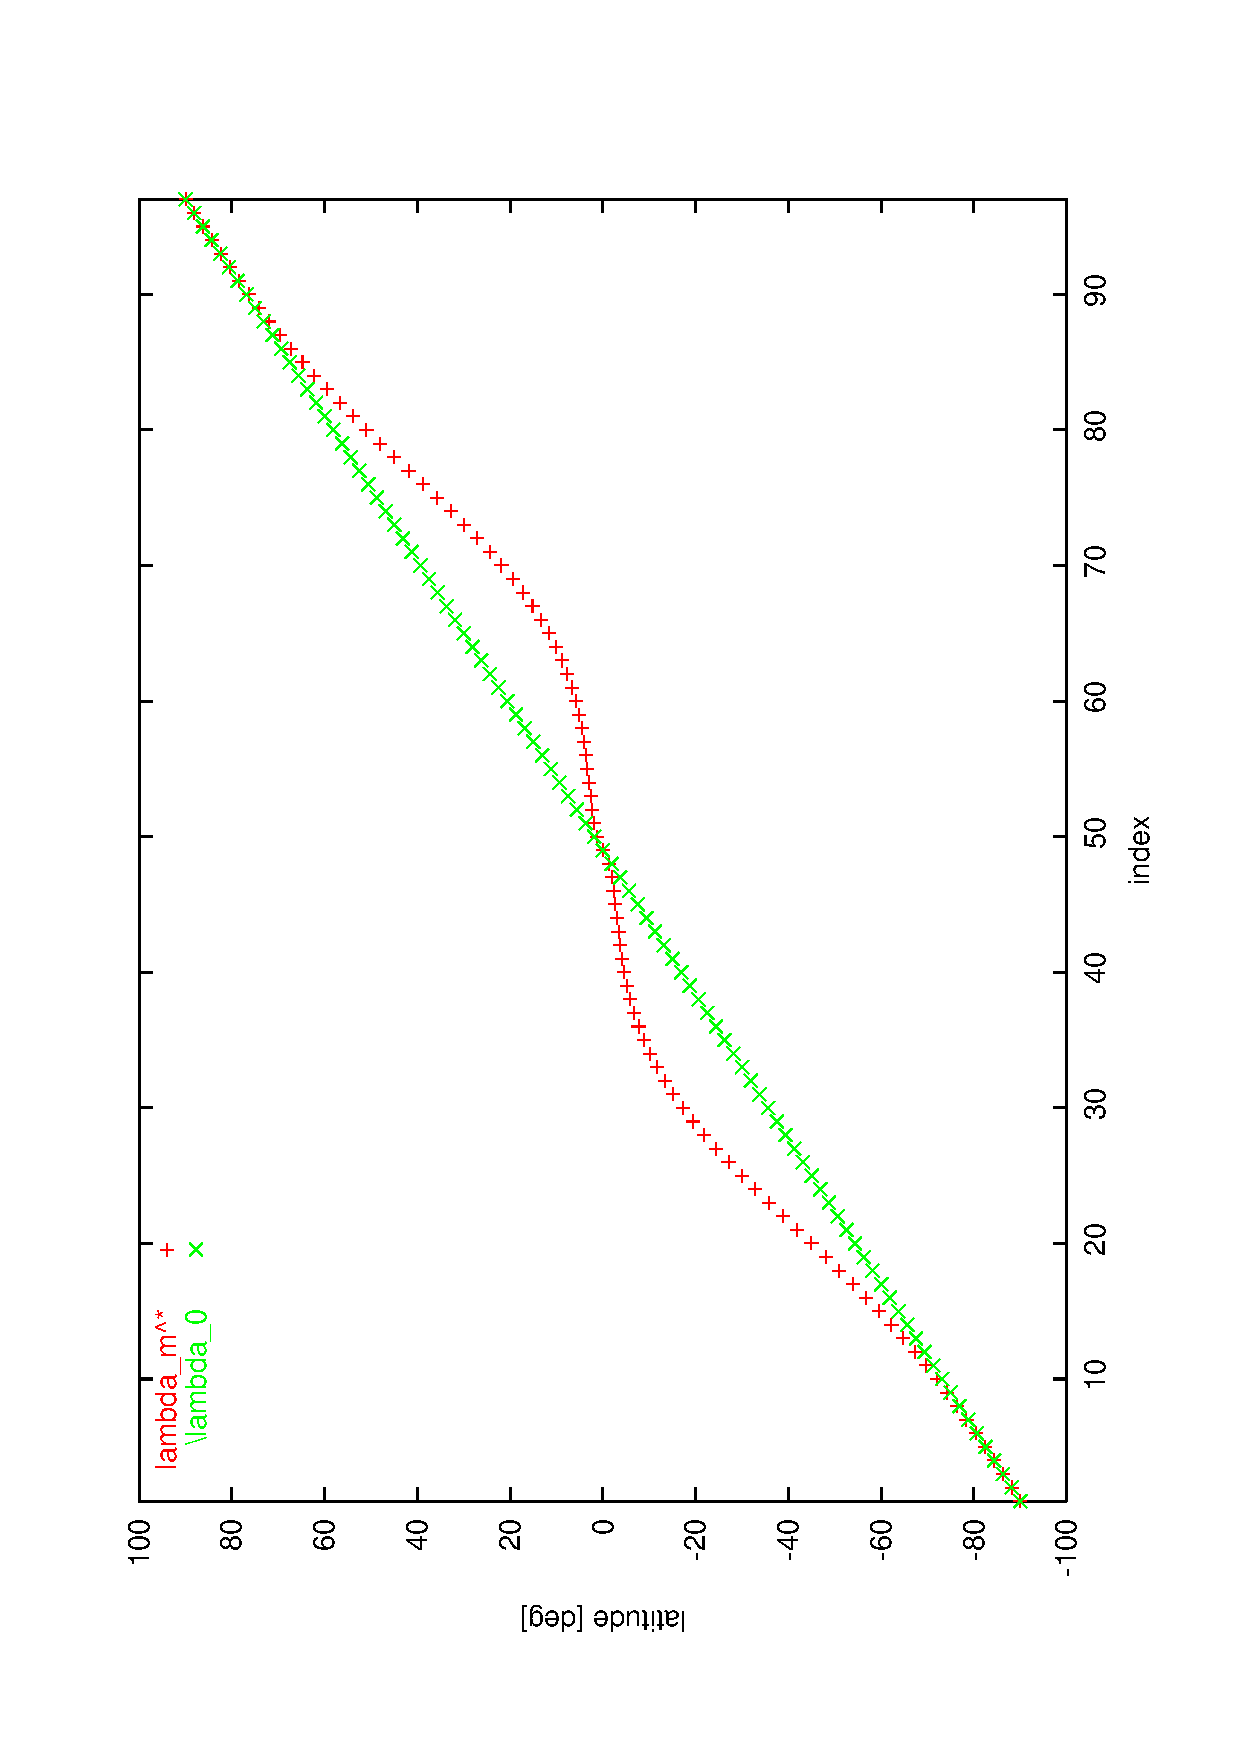
\includegraphics[scale=0.3, angle=-90]{./tex_plot/lambda.epsi}
  \caption{Distribution of modified apex latitude points for $\lambda_0$
  (crosses) and 
  $\lambda_m^*$ (pluses)}
   \label{fig:lambda}
\end{figure}
%
%-------------------------------------------------------------------------------------------
\section{Mapping from and to the geomagnetic grid}
%
The fields in table \ref{tab:map_transf} are mapped from the geographic grid 
to the geomagnetic
grid in \src{subroutine transf}. \src{Subroutine transf} is called from 
\src{subroutine dynamo} once per
timestep.
%
\begin{table}[tb]
\begin{tabular}{|p{3.0cm} ||c|c|c|c|c|c|} \hline
 variable                                  & description            & unit & dimension \\ \hline \hline
%
$\sigma_P$                                 & Pedersen conductivity   & S/m & 3D   \\ 
$\sigma_H$                                 & Hall conductivity       & S/m & 3D   \\
z                                          & geopotential height     & cm & 3D   \\ 
$sin I_m(h_0)$                             & inclination angle       & -  & 2D   \\ 
$B_{e3}(h_0)$                                     & magnetic field component    & T  & 2D   \\
$\frac{\mathbf{d}_1 \cdot \mathbf{d}_2}{D}(h_0)$  & base vector quantity	& - &  2D   \\ 
$\frac{\mathbf{d}_1 \cdot \mathbf{d}_1}{D}(h_0)$  & base vector quantity	& - &  2D   \\
$\frac{\mathbf{d}_2 \cdot \mathbf{d}_2}{D}(h_0)$  & base vector quantity	& - &  2D   \\
${u}_{e1}, {u}_{e2} $                     & neutral wind components & $\frac{m}{s}$ & 3D   \\ \hline
%
\end{tabular}
\caption{Mapped fields in \src{subroutine transf}}
\label{tab:map_transf}
\end{table}  
%
The lower boundary of the TIEGCM model (up to version 1.8) 
is at 97 km, however the field
line integration starts at $h_0=$ 90 km altitude, where the lower boundary 
of the
ionosphere is assumed to lie. Therefore the fields in table \ref{tab:map_transf} 
needed for the field line integration
have to be
extended downward. 
Three additional height levels (k=-2 to 0) are introduced with k being the
height index. The geopotential height $z$ is linearly
extrapolated and the conductivities are assumed to vary exponentially.
%
\begin{alignat}{2}
  z(k)               &= h_0+(k+2)
                \bigl(\frac{z(k=1)-h_0}{3} \bigr) \quad &\text{for k=0 to -2 by -1}  \\
  {\sigma}_{P}(k')  &= {\sigma}_{P}(k'=1)
                exp \bigl(\frac{z(k+\frac{1}{2})-z(k=1\frac{1}{2})}{ fac_{ped}}
		\bigr)\quad &\text{for k' =0 to -2 by -1} \label{eq:condped_ext}   \\
  {\sigma}_{H}(k') &= {\sigma}_{H}(k'=1)
                exp \bigl(\frac{z(k+\frac{1}{2})-z(k=1\frac{1}{2})}{ fac_{hall}}
		\bigr) \quad &\text{for k' =0 to -2 by -1} \label{eq:condhall_ext}   
\end{alignat}
% 
Note that the geopotential height is saved on full pressure levels (k) and 
the conductivities on half pressure levels ($k'=k+\frac{1}{2}$). 
Therefore the geopotential height $z$ for
the conductivity extension (eq. \ref{eq:condped_ext} and 
\ref{eq:condhall_ext}) is calculated at half pressure levels denoted by e.g.
$k'=k+\frac{1}{2}$. The factors at which the conductivities are assumed to decay
below the lower boundary of the model are $fac_{ped}= 5. \times 10^5$ and 
$fac_{hall}= 3. \times 10^5$ \\

The neutral winds $\mathbf{u}$ are assumed to be constant between $h_0$=90 
to 97 km and
can be expressed by
%
\begin{equation}
   \mathbf{u} = \mathbf{e}_1 u_{e1} + \mathbf{e}_2 u_{e2}
\end{equation}
%
with the base vectors $\mathbf{e}_i$  (see \cite{rich95}).
The base vectors $\mathbf{d}_i$ and $\mathbf{e}_i$ satisfy
$\mathbf{d}_i \mathbf{e}_j = \delta_{ij}$ with $\delta_{ij}$ the Kronecker
delta. The components $u_{e1}$
in magnetic eastward and  $u_{e2}$ in down--/equatorward direction at altitude
$h$  are  calculated by 
%
\begin{align}
  u_{e1}(h) &= \mathbf{d}_1(h) \cdot \mathbf{u}(h) \\
  u_{e2}(h) &= \mathbf{d}_2(h) \cdot \mathbf{u}(h)
\end{align}
% 
The height variation of $\mathbf{d}_1(h)$ and $\mathbf{d}_1(h)$ is determined by 
%
\begin{align}
  \mathbf{d}_1(h) &= \bigl[\frac{R_E+h_0}{R_E+h)} \bigr]^{3/2} \mathbf{d}_1(h_0)\label{eq:vary_h_d1} \\
  \mathbf{d}_2(h) &= \bigl[\frac{R_E+h_0}{R_E+h)}\bigr]^{3/2}
      \sqrt{\frac{4.-3. cos^2\lambda_m(h_0)}{(4.-3. \frac{R_E+h_0}{R_E+h} 
      cos^2\lambda_m(h_0)}} \mathbf{d}_2(h_0) \label{eq:vary_h_d2}	    
\end{align}
%
with $\lambda_m(h_0)$ the modified apex value at height $h_0$ which is kept 
constant vertically and thus representing the quasi--dipole latitude.
%
In addition the following quantities are calculated
%
\begin{align}
  \frac{\mathbf{d}_1 \cdot \mathbf{d}_1}{D} \\
  \frac{\mathbf{d}_2 \cdot \mathbf{d}_2}{D} \\
  \frac{\mathbf{d}_1 \cdot \mathbf{d}_2}{D}
\end{align}
% 
These values are calculated at height $h_0$. The values at the pole need special
 treatment
since we have different longitudinal grid points for one spatial point. 
Therefore the pole values are
extrapolated from the longitudinal averaged values next to the pole.
%
\begin{equation}
   x(l_{pole}) = \frac{9 \sum_{lon} x(l_{pole} \pm 1)-\sum_{lon} x(l_{pole} \pm 2)}
      {8 \; nlon}
\end{equation}
%
with the latitudinal index of the pole $l_{pole}$ and $x(l_{pole} \pm 1)$ denoting
the values one grid point off the south-- and northpole respectively. The number of
geographic longitudinal grid points is $nlon$ and $\sum_{lon}$ denotes the sum over all
longitudinal grid points. The following
fields are processed: $z(h)$, $\sigma_P(h)$, ${\sigma}_{H}(h)$, $u_{e1}(h)$, 
$u_{e2}(h)$,
$\frac{\mathbf{d}_1 \cdot \mathbf{d}_1}{D}$, $\frac{\mathbf{d}_2 \cdot \mathbf{d}_2}{D}$, 
$\frac{\mathbf{d}_1 \cdot \mathbf{d}_2}{D}$, $sin I_m$, $B_{e3} $. In addition, periodic
points for these fields are added.

%
The mapping from the geographic to the geomagnetic grid is done for each latitude
separately right before the integration along the field line which foot point at
this latitude. 
The field line integration is described in section 
\ref{cap:fieldlineintg}. The geomagnetic equatorial values 
$\sigma_{P, eq}(h)$, ${\sigma}_{H, eq}(h)$, $u_{e1, eq}(h)$, $u_{e2, eq}(h) $ 
have to be known at each geomagnetic
latitude and therefore are calculated before the field line integration 
is done. The mapping from the geographic to the geomagnetic grid
is done by a  bilinear interpolation. The surrounding geographic grid points
for each geomagnetic grid point and the weighting factors for each of the
geographic points are determined in \src{subroutine apxparm}.



%
\section{High Latitude Input}\label{cap:high_lat}
%
\subsection{Weimer}
%
To use the high latitude potential as defined by
Weimer the flag \flags{POTENTIAL\_MODEL = WEIMER} in the input file of a TIEGCM 
has to be set. However the Weimer high latitude
potential is not working in the version 1.7 and 1.8 of 
TIEGCM. Please check newer version carefully. 
%
\subsection{Heelis}
%
At high latitude the electric potential pattern can be prescribed as
determined by Heelis. The calculation of the
electric potential due to Heelis is not described since we didn't work
on this part of the code. The Heelis potential pattern is the
default if the flag \flags{POTENTIAL\_MODEL} is not specified. 
The Heelis model is also the
basis for the high latitude modifications described in the following
sections. Therefore when using these modifications the flag  
\flags{POTENTIAL\_MODEL = HEELIS} should be set in the input file. 
%
\subsection{Modification of the high latitude input}
%
In the electrodynamo equation (\ref{eq:edyn}) we neglected so far the
 current part $J_{Mr}$ between the ionosphere and magnetosphere. The current
from the magnetosphere can be influenced by the electric field
distribution, however the mechanism is not fully understood. The total field-aligned
current between ionosphere and magnetosphere can be described as the divergence
of a magnetospheric current $\mathbf{K}^M$
%
\begin{equation}
   {J}_{Mr}  = \frac{1}{R_0 cos \lambda_m} \bigl(
    \frac{\partial K_{\phi}^M}{\partial \phi_m} + 
    \frac{\partial K_{|\lambda|}^M cos \lambda_m}{\partial | \lambda_m| } \bigr) 
    \label{eq:magcurrent}
\end{equation}
%
The height integrated current density $\mathbf{K}^M$ doesn't have 
to be realistic, but the divergence, i.e. the current $J_{Mr}$,
should be. Using the divergence assures that the integrated field-aligned
current over both hemispheres vanishes, and therefore there is no net current into the
ionosphere. The two components of the field-aligned
current $K_{\phi}^M$ and $K_{|\lambda|}^M$, eastward and poleward/ upward, 
can be differently defined depending on the acting region and the
mimicking mechanism. The different contributions 
are described in the following three subsections. Note that in the
default code non of these options is used. To use them one or all
of the flags
\flags{mod\_heelis}, \flags{J\_rR} and \flags{eqMgCnd} have to be set to 
\src{.true.} in the  \src{dynamo\_module}.
%.
\subsubsection{Field--aligned current}\label{cap:fldalg_curr}
%
This part has not been tested yet, however the source code can be found in 
\src{subroutine calrhs\_jrr}. To use the field--aligned part 
the flag  \src{J\_rR = .true.} 
in  \src{dynamo\_module} has to be set. 
The magnetospheric current components $K_{\phi}^M$ and 
$K_{|\lambda|}^M$ for the field--aligned current can be derived 
from a reference potential 
$\Phi_R$ which we assume is the Heelis potential for now. Using the
Heelis potential leads to realistic magnitudes and directions 
in the current, but
might not represent correctly the field-aligned current in the region 1.
%
\begin{align}
  K_{\phi}^M       &=  \frac{f_{\lambda}}{R_0} \bigl( \frac{\Sigma_{\phi \phi}^T}{cos
   \lambda_m} \frac{\partial \Phi_R}{\partial \phi_m} + 
   \Sigma_{\phi \lambda}^T \frac{\partial \Phi_R}{\partial |\lambda_m|} \bigr) \label{eq:fac_phi}\\
  K_{|\lambda|}^M  &= \frac{f_{\lambda}}{R_0 cos \lambda_m} \bigl( \Sigma_{\lambda \phi}^T
    \frac{\partial \Phi_R}{\partial \phi_m} + 
   \Sigma_{\lambda \lambda}^T cos \lambda_m 
   \frac{\partial \Phi_R}{\partial |\lambda_m|} \bigr) \label{eq:fac_lam}
\end{align}
%
The factor $f_{\lambda}$ is set such that it's 1 poleward of the the convection reversal
boundary $ \lambda_m^{crb}$ and zero equatorward. Thus, the current 
represents region 1 current and is zero in the region 2.
%
\begin{align}
  f_{\lambda} = 1 \quad \text{for} \quad |\lambda_m| \ge  \lambda_m^{crb} \\ 
  f_{\lambda} = 0 \quad \text{for} \quad |\lambda_m| <  \lambda_m^{crb} 
\end{align}
%
In TIEGCM the value for the convection reversal boundary $ \lambda_m^{crb}$  
is set to $75^o$ in the
\src{module cons}. Note that this is not a physical meaningful value since 
the convection reversal boundary is fixed.
For the modified reference potential in section \ref{cap:modrefpot} 
a variable value for the convection reversal boundary will
be used which is set in the \src{aurora module}. 
The current components in equations (\ref{eq:fac_phi}) and (\ref{eq:fac_lam})
are calculated in a similar way as the left hand side of the electrodynamo 
equation, which is described in section
\ref{chap:finitediff}. The conductance expressions in equation 
(\ref{eq:sig_dif1})--(\ref{eq:sig_dif4}) are used to calculate the current 
components in equations (\ref{eq:fac_phi}) and (\ref{eq:fac_lam}), and therefore
these conductances are input to the 
\src{subroutine calrhs\_jrr} where the current components eq. 
(\ref{eq:sig_dif1})--(\ref{eq:sig_dif4}) are calculated. 
The finite difference stencil for the partial derivatives in equations 
(\ref{eq:fac_phi}) and (\ref{eq:fac_lam})  is set up in  
\src{subroutine nsstencil}. In comparison to the set up of the finite difference 
stencil in section
\ref{chap:finitediff} for the left hand side of the electrodynamo equation, 
here, it's done for both hemispheres and 
without upwinding technique. Once the finite difference stencil is calculated 
the electric
potential $\Phi_R$ is inserted, which is done in \src{subroutine insert\_pot}, 
to calculate the
current components. Although the calculation is done for both hemisphere, 
it is not necessary since the used Heelis potential
is symmetric about the equator and the coefficients of the conductances in equations 
(\ref{eq:sig_dif1})--(\ref{eq:sig_dif4}) are already the sum of the two
hemispheres. After calculating the current it is added to the right hand side of the
electrodynamo equation (\ref{eq:edyn}).
%
\subsubsection{Equivalent magnetospheric conductances}\label{cap:magncond}
%
The magnetospheric field-aligned current can be influenced by the electric field
distribution in the ionosphere, and therefore depend on the electric potential. The
region 2 current with the shielding effect of strong electric fields from high to low
latitude is an example of this magnetosphere--ionosphere interaction. The region 2
current can be approximated by a Hall conductor. In addition, the 
magnetospheric ion loss
can be simulated by adding a zonal Pedersen conductance. 
In TIEGCM we adopt the concept from
\cite{peym93} by using equivalent magnetospheric conductances 
$\Sigma_{\phi \phi}^M$ and $\Sigma_{H}^M$. 
The magnetospheric current in eq. (\ref{eq:magcurrent}) can
be replaced by
%
\begin{align}
  K_{\phi}^M       &=  \frac{-1}{R_0} \bigl( \frac{\Sigma_{\phi \phi}^M}{cos
   \lambda_m} \frac{\partial \Phi}{\partial \phi_m} + 
   \Sigma_{H}^M \frac{\partial \Phi}{\partial |\lambda_m|} \bigr)  \label{eq:mageqcur_phi}\\
  K_{|\lambda|}^M  &=   \frac{\Sigma_{H}^M}{R_0 cos \lambda_m}
    \frac{ \partial \Phi_R}{\partial \phi_m} \label{eq:mageqcur_lam}
\end{align}
%
with $\Sigma_{\phi \phi}^M$ and $\Sigma_{H}^M$ being the equivalent magnetospheric zonal
Pedersen and Hall conductances. The values of $\Sigma_{\phi \phi}^M$ and $\Sigma_{H}^M$
are taken from figure 4 in \cite{peym93} and plotted in figure \ref{fig:magcond}. In 
\src{subroutine set\_cicr} the equivalent magnetospheric conductances 
are set up and added to the conductances due to solar ionization and
particle precipitation in \src{subroutine add\_cicr}. In figure 
\ref{fig:magcond} the equivalent magnetospheric
conductances start at $72^o$ magnetic latitude which is the 
convection reversal boundary for this specific
case. However, the convection reversal boundary varies with the geomagnetic conditions
and the location is determined in the \src{aurora module}. 
The contributions to the electrodynamo equation 
due to the equivalent magnetospheric conductances 
 are calculated in a similar way as
described in section \ref{cap:fieldlineintg} for the left hand side of the electrodynamo
equation. The conductances are calculated on the irregular spaced grid $\lambda_m^*$, 
but for the finite differencing the regular grid $\lambda_0$ in
 $\lambda_m^*$ is used. Therefore, the
difference in the partial derivatives due to the change from  $\lambda_m^*$ to  $\lambda_0$ 
have to be taken into account,
as described in table 
\ref{tab:transf_quantities}. The conductance quantities are then
 prepared for the finite differencing as shown in eq. 
(\ref{eq:sig_dif1}) and (\ref{eq:sig_dif3}) and added to the conductances due to solar
ionization and particle precipitation. To use the equivalent magnetospheric
conductances, the flag \flags{eqMgCnd} has to be set to 
\src{.true.} in the  \src{dynamo\_module}. 
%
\begin{figure}
  \centering
  \includegraphics[scale=0.3, angle=-90]{./tex_plot/magcond.epsi}
  \caption{Latitudinal variation of equivalent magnetospheric conductances 
    $\Sigma_{\phi \phi}^M$ ($C_r$) and $\Sigma_{H}^M$ ($C_i$) for the 
    convection reversal boundary at $72^o$.}
   \label{fig:magcond}
\end{figure}
%
\subsubsection{Modified reference potential}   \label{cap:modrefpot}
%
In the region 1 the magnetospheric current in eq.(\ref{eq:magcurrent}) can be represented
by the combination of a field--aligned current described in 
section \ref{cap:fldalg_curr} and a reference electric potential 
distribution $\Phi^R$. The later is described in
the following. The contribution to the magnetospheric current from a reference potential
can be specified by
%
\begin{align}
  K_{\phi}^M       &=  \frac{\Sigma^R}{R_0 cos
   \lambda_m} \frac{\partial (\Phi^R - \Phi)}{\partial \phi_m} \label{eq:refpotphi}\\
  K_{|\lambda|}^M  &=   \frac{\Sigma^R}{R_0 }
    \frac{\partial (\Phi^R - \Phi) }{\partial \phi_m} \label{eq:refpotlam}
\end{align}
%
The reference conductance $\Sigma^R$ is not a physical conductance, but determines how
strongly the calculated electric potential $\Phi$ reflects the reference potential
$\Phi^R$. The reference conductance is set to
%
\begin{align}
  \Sigma^R =& \text{min} \; \bigl( {\Sigma_{max}^R,\Sigma_b [ e^{|\lambda_m-\lambda_{crb}|
          \frac{2}{\alpha_t}}-1]}  \bigr) \quad \text{for} \quad |\lambda_m|
	   \ge  \lambda_m^{crb} \label{eq:sigmar1}\\ 
  \Sigma^R =& 0 \quad \text{for} \quad |\lambda_m| <  \lambda_m^{crb} \label{eq:sigmar2}
\end{align}
%
with $\alpha_t$ being the width of the transition zone, here $3^o$, equatorward of the
convection reversal boundary $\lambda_m^{crb}$. 
The maximum reference conductance 
$\Sigma_{max}^R$ is set to $10,000 \; S$ and the base conductance $\Sigma_b$ 
is 5 S. In the
polar cap region the electric potential should be the reference potential. In the source
code the Heelis potential is used for the reference
potential $\Phi^R$. The convection reversal boundary is denoted by $\lambda_m^{crb}$, 
which varies with the geomagnetic conditions, and is set in the \src{aurora module}.
In figure \ref{fig:sigma_r} the latitudinal variation of the
reference conductance $\Sigma^R$ is shown for $\lambda_m^{crb} = 72^o$. 
\\

In the source code the calling tree is the
following
%
\begin{verbatim}
subroutine dynamo
...
if (mod_heelis) then
   if(istep = 1 ) then call set_zigmar
   call add_zigmar
   call diff_rimr
   call add_rimr
endif
...
\end{verbatim}
%
To use the modified reference potential the flag 
\flags{mod\_heelis} in the  \src{dynamo\_module} has to be set to \src{.true.}. 
The current in the equations (\ref{eq:refpotphi}) and (\ref{eq:refpotlam})
are calculated like the left hand side of the electrodynamo equation 
which is described in section
\ref{chap:finitediff}. The reference conductances 
$\Sigma^R$ are calculated according to eq. (\ref{eq:sigmar1}) and 
(\ref{eq:sigmar2}) in \src{subroutine set\_zigmar}. 
The coefficients of the reference conductance are added 
in \src{subroutine add\_zigmar} to the conductances 
$\Sigma_{\phi \phi}$ and $\Sigma_{\lambda \lambda}$ of the electrodynamo equation.
The finite difference stencil is set up in
\src{subroutine diff\_rimr} by
\src{subroutine nsstencil}. In comparison to the set up of the stencil for 
the left hand side of the electrodynamo equation, in section
\ref{chap:finitediff}, the stencil is calculated for both hemispheres and no
upwinding technique are used. Once the finite difference stencil is 
calculated the electric
potential $\Phi_R$ is inserted to calculate the additional 
current for the right hand side of the electrodynamo equation
in \src{subroutine insert\_pot}. Although the additional current
is determined  for both hemisphere separately,
this is not necessary since the reference  potential and the coefficients 
of $\Sigma^R$
are symmetric about the equator.
%
%
\begin{figure}
  \centering
  \includegraphics[scale=0.3, angle=-90]{./tex_plot/sigma_r.epsi}
  \caption{Latitudinal variation of reference conductance 
    $\Sigma^R$ for  $\lambda_m^{crb}= 72^o$  }
   \label{fig:sigma_r}
\end{figure}
%
%

%
%
\section{Field line Integration}\label{cap:fieldlineintg}
%
This section refers to the \texttt{subroutine fieldline\_integrals} in TIEGCM. \\
%

The electrodynamo equation is reduced to two dimensions
assuming that the field--lines
are equipotential due to the high conductivity along the field--line.
The variable along the field line is $s$, and ${s_L}$ and ${s_U}$ are
the lower and upper boundary
of the line--integration. The inclination of the geomagnetic field--line at the
reference height $h_0$ on an assumed spherical Earth is $I_m$, and $B_{e3}$ is 
the component of the geomagnetic field along the field--line. Note that all value,s except
the geopotential height $z$, are stored on half pressure levels to make the integration more
convenient. \\
%
\begin{figure}
  \centering
  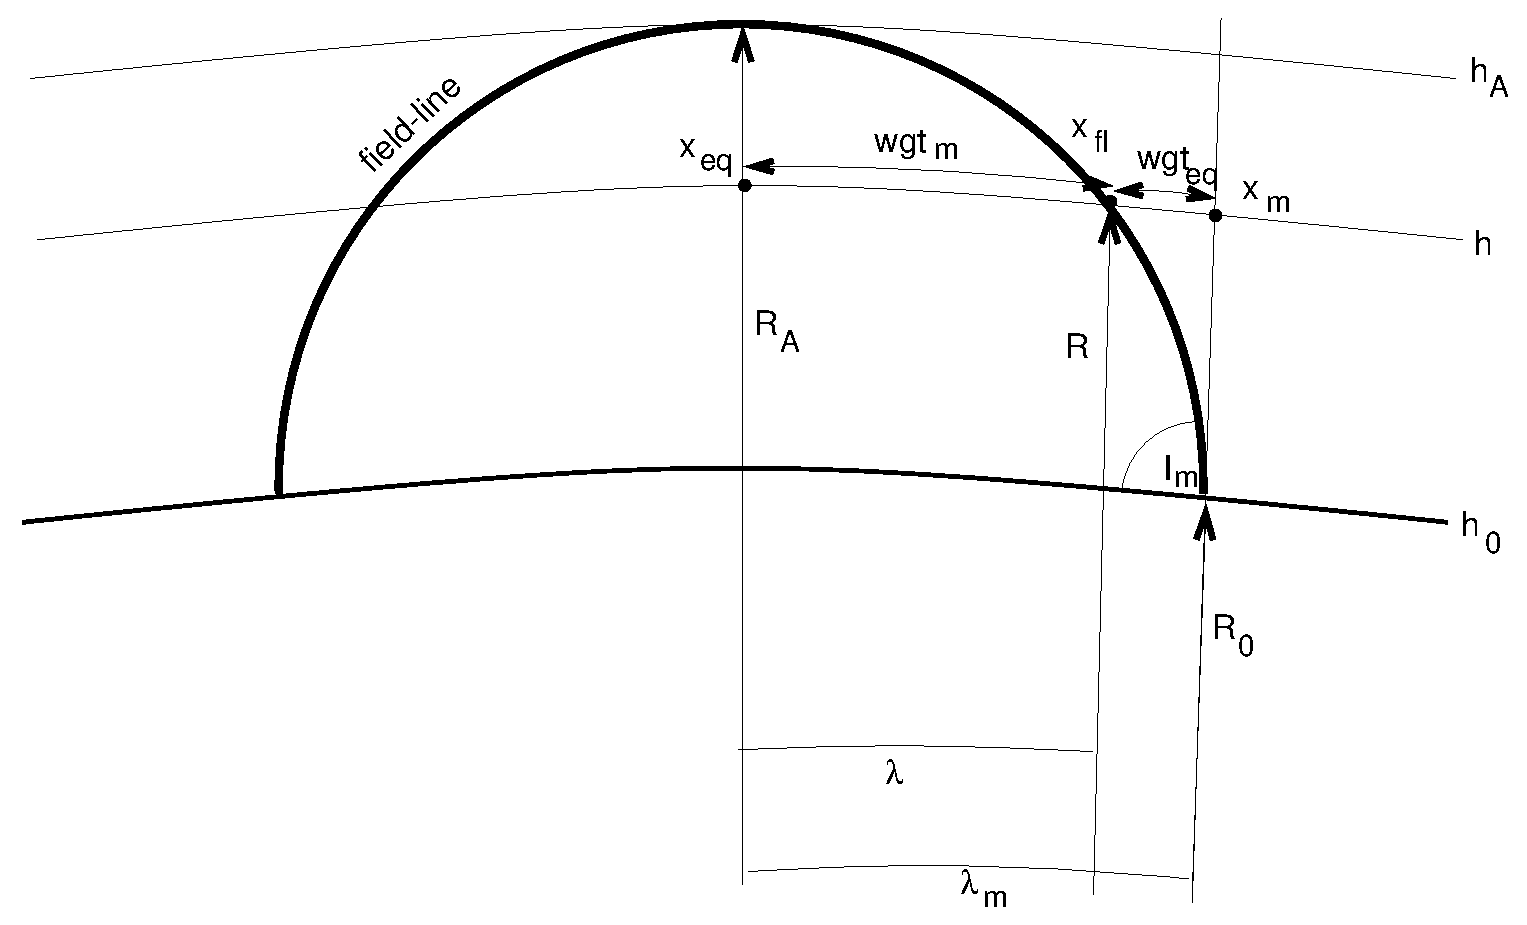
\includegraphics[scale=0.3]{./tex_plot/fl_geometry.eps}
  \caption{Sketch of geometry for the field--line integration}
   \label{fig:fieldline_intg}
\end{figure}
%
\paragraph{Approximation of field line values}
%
The correct way to do the field line integration would be to trace points along
the field line. However, the geomagnetic grid in TIEGCM is not oriented along the field line,
and therefore the tracking
would involve a two dimensional search and an interpolation to calculate the value on the field
line. This can be computational expensive and therefore an approximation, which should be close
to the true field line integration, is used.
The field line integration is approximated by a height integration 
combined with an interpolation
between the height-varying values at the foot point of the field line ($\lambda_m$, h) and the magnetic 
equator ($\lambda_m = 0, h$) (see. figure  \ref{fig:fieldline_intg}). Hence, only the height varying values at the foot point location 
$(\lambda_m, h)$ are needed.
Figure \ref{fig:fieldline_intg} shows schematically
a field line with the foot point latitude $\lambda_m$ at the reference height $h_0$. The
value $x_{fl}$ at height $h$ on the field line is approximated by the 
value $x_{eq}$ at the equator and height h
and the value $x_m$ at foot point latitude $\lambda_m$ and height h.
%
\begin{equation}
 x_{fl} = wgt_{eq} x_{eq} + wgt_m x_m \label{eq:approx_fl}
\end{equation}
%
with the weights $wgt_{eq}$ for the equator value and $wgt_{m}$  for the foot point value. 
From figure \ref{fig:fieldline_intg} the weight can be found as
%
\begin{equation}
 wgt_{eq} = \frac{\lambda_m -\lambda}{\lambda_m} \approx  
            \frac{sin(\lambda_m -\lambda)}{\lambda_m} \label{eq:wgh1}
\end{equation}
%
assuming that the difference $\lambda_m -\lambda$ is small, which is true close to the
foot point of the field line. Note that determining $\lambda$ would involve searching for the
point on the field line at height h which is time consuming, thus the sinus is used.
For field lines which foot point is at mid-- and height latitude the value on the
field line is essentially the height--varying value at the foot point, since the field line is
almost vertical.
Close to the magnetic equator the approximation is not so good anymore but the inaccuracy 
can be neglected when compared to the total field line integration.
 The term
$sin(\lambda_m -\lambda)$ can be substituted by
%
\begin{equation}
 sin(\lambda_m -\lambda) = sin \lambda_m cos \lambda - cos \lambda_m sin \lambda \label{eq:wgh2}
\end{equation}
%
and since for a dipolar field $R = R_A cos^2 \lambda$ the $cos \lambda$ and 
$sin \lambda$ in equation (\ref{eq:wgh2}) can be substituted by 
%
\begin{alignat}{2}
   cos \lambda =& \sqrt{\frac{R}{R_A}};   \quad
   sin \lambda =& \sqrt{1-\frac{R}{R_A}};  \\
   cos \lambda_m =& \sqrt{\frac{R_0}{R_A}};   \quad
   sin \lambda_m =& \sqrt{1-\frac{R_0}{R_A}}; 
\end{alignat}
%
with $R_A$ the radius of the field--line apex (see figure \ref{fig:fieldline_intg}). 
The weighting factors are 
%
\begin{align}
 wgt_{eq} &\approx \frac{1}{\lambda_m} \sqrt{1-\frac{R_0}{R_A}}\sqrt{\frac{R}{R_A}}
     - \sqrt{\frac{R_0}{R_A}}\sqrt{1-\frac{R}{R_A}} \\
 wgt_{m}  &= 1- wgt_{eq}
\end{align}
%
The quantities on the
field--line  at ($h,\lambda$) are therefore approximated by
%
\begin{align}
 \sigma_{P}(h,\lambda) &= wgt_{eq}(h,\lambda_{eq})\sigma_{P}(h,\lambda_{eq})  + 
          wgt_m(h,\lambda_m) \sigma_{P}(h,\lambda_m) \label{eq:approx_sig1} \\
 \sigma_{H}(h,\lambda) &= wgt_{eq}(h,\lambda_{eq})\sigma_{H}(h,\lambda_{eq})  + 
            wgt_m(h,\lambda_m) \sigma_{H}(h,\lambda_m) \label{eq:approx_sig2}\\
 {u}_{e1}(h,\lambda) &= wgt_{eq}{u}_{e1}(h,\lambda_{eq})(h,\lambda_{eq})  + 
          wgt_m(h,\lambda_m) {u}_{e1}(h,\lambda_m) \label{eq:approx_ue1} \\
 {u}_{e2}(h,\lambda) &= wgt_{eq}{u}_{e2}(h,\lambda_{eq})(h,\lambda_{eq})  + 
            wgt_m(h,\lambda_m) {u}_{e2}(h,\lambda_m) \label{eq:approx_ue2}
\end{align}
%
\paragraph{Height variation of $\mathbf{d}_1$ and $\mathbf{d}_2$ }
%
The apex values $\frac{d_1^2}{D}$, $\frac{d_2^2}{D}$ and $\frac{\mathbf{d}_1 \cdot
\mathbf{d}_2}{D}$ are referenced to height $h_0$ (see section \ref{cap:apex_coord}). 
The height variation of these values are
small, but should be taken into account. The values $\mathbf{d}_1$, $\mathbf{d}_2$
and $D$ vary with height like
%
\begin{align}
   \mathbf{d}_1^2(h) &= \bigl[ \frac{R_0}{R} \bigr]^3 \mathbf{d}_1^2(h_0)\\
   \mathbf{d}_2^2(h) &= \bigl[ \frac{R_0}{R} \bigr]^3 \bigl[ 
	   \frac{4-3cos^2 \lambda}{4-3 \frac{R_0}{R} cos^2 \lambda} \bigr]\mathbf{d}_2^2(h_0) \\
   D(h) = \mathbf{d}_1 \cdot \mathbf{d}_2
	      &= \bigl( \frac{R_0}{R} \bigr)^3  \bigl(\frac{4-3cos^2 \lambda}
		     {4-3 \frac{R_0}{R} cos^2 \lambda} \bigr)^{1/2} D(h_0)
\end{align}
%
Using the dipole approximation $cos^2 \lambda = \frac{R}{R_A}$ we can approximate
the height variation by
%
\begin{align}
   \frac{\mathbf{d}_1^2(h)}{D(h)} &= \bigl( \frac{R_A-\frac{3}{4} R_0}
                     {R_A-\frac{3}{4} R} \bigr)^{1/2}\frac{\mathbf{d}_1^2(h_0)}{D(h_0)} = 
		     \frac{1}{h_{fac}}\frac{\mathbf{d}_1^2(h_0)}{D(h_0)}
		     \label{eq:d_hgt1a}\\
   \frac{\mathbf{d}_2^2(h)}{D(h)} &= \bigl(\frac{R_A-\frac{3}{4} R}
                     {R_A-\frac{3}{4} R_0} \bigr)^{1/2}\frac{\mathbf{d}_2^2(h_0)}{D(h_0)}  = 
		     h_{fac}\frac{\mathbf{d}_2^2(h_0)}{D(h_0)}  \label{eq:d_hgt1b}
\end{align}
%
%
\paragraph{Approximation of ds along the field line}
%
Since the integration is done in height rather than along the field--line
$ds$ in equations (\ref{eq:eldy_3})--(\ref{eq:eldy_8}) is expressed in terms of height h.
%
\begin{equation}
   ds =  \frac{dh}{|sin I|}\label{eq:ds1}
\end{equation}
%
However, $sin I$ is going to zero at the magnetic equator and ds would be infinite.
Therefore, we have to approximate the relation in equation (\ref{eq:ds1}). 
Starting from the calculation
of $sin I$ and using the dipole approximation $cos^2 \lambda = \frac{R}{R_A}$ leads to
%
\begin{equation}
   sin I  = \frac{2 sin \lambda}{\sqrt{4-3cos^2 \lambda}} = 
            2 \sqrt{\frac{ h_A - h}{R_E + 4 h_A - 3h}} \label{eq:ds3a}
\end{equation}
%
The numerator $\sqrt{ h_A - h}$ varies more than the denominator. Therefore equation 
(\ref{eq:ds1}) is written as
%
\begin{equation}
   ds  = \frac{dh}{|sin I|} = -A(h) d \sqrt{h_A-h} = 
         \frac{A(h) dh}{2 \sqrt{h_A-h}}\label{eq:ds1b}
\end{equation}
%
with $A(h)$ is the area at height h.
The minus sign is introduced since ds should increase with increasing height.
From equation (\ref{eq:ds1b}) follows that the area A(h) and $A(h_0)$ at the reference height is
%
\begin{equation}
   A(h)   = \frac{2 \sqrt{h_A-h}}{|sin I|};  \quad
   A(h_0) = \frac{2 \sqrt{h_A-h_0}}{|sin I_m|};  \label{eq:ds2}
\end{equation}
%
Thus, the height varying factor is
%
\begin{equation}
   \frac{A(h)}{A(h_0)}   = \frac{2 \sqrt{h_A-h}}{|sin I|} \frac{|sin I_m|}{2 \sqrt{h_A-h_0}} =
    \sqrt{\frac{R_A - \frac{3}{4} R}{R_A - \frac{3}{4} R_0}} \label{eq:ds3b}
\end{equation}
%
substituting the inclination angle $sin I$ and $sin I_m$ from equation (\ref{eq:ds3a}).
Inserting equation (\ref{eq:ds2}) for $A(h_0)$ in equation (\ref{eq:ds1b}) will
give 
%
\begin{equation}
     {A(h)}   = \frac{2 \sqrt{h_A-h_0}}{|sin I_m|}
     \sqrt{\frac{R_A - \frac{3}{4} R}{R_A - \frac{3}{4} R_0}} = A(h_0) h_{fac} \label{eq:ds7}
\end{equation}
%
The height varying factor $A(h)$ consists of two terms:
a height dependent factor $h_{fac}$ which was already defined in equation (\ref{eq:d_hgt1b}) and
a height independent term $A(h_0)$. \\
%
The factor $- d \sqrt{h_A-h}$ in equation (\ref{eq:ds1}) at the pressure level k
 can be discretized as follows
%
\begin{equation}
 - d_k \sqrt{h_A-h} = \sqrt{h_A - h_{k}} - \sqrt{h_A - h_{k+1}}   \label{eq:ds8}
\end{equation}
%
with k being the index of the discrete pressure levels. Note that the geopotential height $z$
is used for $h$ which is stored at full pressure levels. 
The increment along the field line in eq. (\ref{eq:ds1b}) can be written as 
%
\begin{equation}
   ds  = - A(h_0) h_{fac} d \sqrt{h_A-h} \label{eq:ds9}
\end{equation}
%
%
\paragraph{Field line integration}
%
The following fields are calculated (see also equations \ref{eq:eldy_1}, \ref{eq:eldy_2}, 
 \ref{eq:eldy_3}, \ref{eq:eldy_4}, \ref{eq:eldy_7}, \ref{eq:eldy_8}) using the field line
 integration
%
\begin{align}
  \frac{\Sigma_{\phi \phi}}{|sinI_m|} &= \int_{s_L}^{s_U}  \frac{ \sigma_{P} \mathbf{d}_1^2}{D}
                 ds \label{eq:fldline_t1}\\
  {|sinI_m|}{\Sigma_{\lambda \lambda}} &= \int_{s_L}^{s_U}  \frac{ \sigma_{P} \mathbf{d}_2^2}{D}
                 ds \label{eq:fldline_t2}\\
  {\Sigma_{C}} &= \int_{s_L}^{s_U}  \frac{ \sigma_{P} \mathbf{d}_1 \cdot \mathbf{d}_2 }{D}
                 ds \label{eq:fldline_t3}\\
  {\Sigma_{H}} &= \int_{s_L}^{s_U}  \sigma_{H}  ds\label{eq:fldline_t4}
\end{align}
%
%
\begin{align}
  \frac{K_{m \phi}^D}{|sinI_m|} &= B_{e3}(h_0) \int_{s_L}^{s_U} \left[ \frac{ \sigma_{P} \mathbf{d}_1^2}{D}
  u_{e2} + \left( \sigma_H - \frac{\sigma_P \mathbf{d}_1 \cdot \mathbf{d}_2}{D} \right) u_{e1}
                \right] ds \label{eq:fldline_t5}\\
  - K_{m \lambda}^D &= \pm B_{e3}(h_0) \int_{s_L}^{s_U} \left[ 
   - \frac{ \sigma_{P} \mathbf{d}_2^2}{D}
  u_{e1} + \left( \sigma_H + \frac{\sigma_P \mathbf{d}_1 \cdot \mathbf{d}_2}{D} \right) u_{e2}
                \right] ds \label{eq:fldline_t6}
\end{align}
%
\begin{table}[tb]
\begin{tabular}{|p{3.0cm} ||c|c|c|c|c|c|} \hline
 quantity               &  name in source code & unit  \\ \hline \hline
%
$\frac{\Sigma_{\phi \phi}}{|sinI_m|}$   & zigm11 &  S  \\ 
${|sinI_m|}{\Sigma_{\lambda \lambda}}$  & zigm22 &  S  \\ 
${\Sigma_{C}}$                          & zigmc  &  S  \\ 
${\Sigma_{H}}$                          & zigm2  &  S  \\ 
$\frac{K_{m \phi}^D}{|sinI_m|}$         & rim(1) & A/m   \\ 
$\pm K_{m \lambda}^D$                   & rim(2) & A/m   \\ \hline
%
\end{tabular}
\caption{Field line integrated quantities in 
\src{subroutine fieldline\_integrals}}
\label{tab:fldline_quantities}
\end{table} 
% 
The field line integration is
approximated by taking  the sum over all pressure level k (k = -2 to \src{mlev}, with
\src{mlev} the number of pressure levels). 
With the approximations of the field line integration in the previous section, the 
integrals in 
equations (\ref{eq:fldline_t1})--(\ref{eq:fldline_t6}) are calculated by
%
\begin{align}
  \frac{\Sigma_{\phi \phi}}{|sinI_m|} &= - A(h_0) \frac{d_1^2}{D}(h_0) 
              \sum_{k=-2}^{mlev} \sigma_{P,k} d_k \sqrt{h_A-h} \\
  {|sinI_m|}{\Sigma_{\lambda \lambda}} &=  - A(h_0) \frac{d_2^2}{D}(h_0) 
              \sum_{k=-2}^{mlev} \sigma_{P,k} h_{fac,k}^2 d_k \sqrt{h_A-h}\\
  {\Sigma_{C}} &= - A(h_0) \frac{\mathbf{d}_1 \cdot \mathbf{d}_2}{D}(h_0) 
              \sum_{k=-2}^{mlev} \sigma_{P,k} h_{fac,k} d_k \sqrt{h_A-h} \\
  {\Sigma_{H}} &= - A(h_0) 
              \sum_{k=-2}^{mlev} \sigma_{H,k} h_{fac,k} d_k \sqrt{h_A-h} 
\end{align}
%
%
\begin{align}
 \begin{split}
  \frac{K_{m \phi}^D}{|sinI_m|} &= - B_{e3}  A(h_0)\sum_{k=-2}^{mlev}
         \bigl[ \sigma_{P,k}\frac{d_1^2}{D}(h_0) u_{e2,k}  +
	  \sigma_{H,k} u_{e1,k}h_{fac,k} -  \\
	  & \sigma_{P,k}
	  \frac{\mathbf{d}_1 \cdot \mathbf{d}_2}{D}(h_0)u_{e1,k}h_{fac,k} \bigr] d_k \sqrt{h_A-h}\\
  - K_{m \lambda}^D &= \pm B_{e3}  A(h_0)\sum_{k=-2}^{mlev}
      \bigl[\sigma_{H,k} u_{e2,k}f_{fac,k} +
        \sigma_{P,k}\frac{\mathbf{d}_1 \cdot \mathbf{d}_2}{D}(h_0)u_{e2,k}h_{fac,k} - \\
	&\sigma_{P,k}\frac{d_2^2}{D}(h_0) u_{e1,k} h_{fac,k}^2
	\bigr] d_k \sqrt{h_A-h}
 \end{split}
\end{align}
%
After the field line integration is carried out the equatorial field line
integral values are set, as well as the equatorial boundary condition is
included. Finally, the coefficients of the partial differential equation are modified 
to take into account that the finite differencing is done with respect to
 the equally spaced grid with $\lambda_0$ which is a function of 
 $\lambda_m^*$, although the derivatives are
 calculated on the irregular grid with  $\lambda_m^*$. 
These tasks are carried out in \texttt{subroutine transf} of TIEGCM and
described in the following. 
%
\paragraph{Equatorial values}
%
The values at the geomagnetic equator are approximated since no field line
integration can be performed. It is assumed that the average along a field line 
for a quantities which primarily
depend on the Pedersen conductivity $\sigma_{P}$ increase by a factor of four
from one field
line to the next higher one. The average along a field line for quantities
mainly dependent on Hall conductivity $\sigma_{H}$ 
vary by 0.83 from one field line to the next higher one. The exact value should
not be important for the electric potential calculation, as long as the values
are physically reasonable and not too different than those of adjacent field
lines. The factor of $\frac{1}{2}$ is introduced to take the adding of the two
hemispheres into account, which is done later.
%
\begin{align}
  \frac{\Sigma_{\phi \phi, eq}}{|sinI_m|} &= 
       \frac{1}{2}\frac{1}{4}\frac{\Sigma_{\phi \phi, eq+\Delta \lambda_m}}{|sinI_m|} \\
  {|sinI_m|}{\Sigma_{\lambda \lambda, eq}} &=  
       \frac{1}{2}\frac{1}{4}{|sinI_m|}{\Sigma_{\lambda \lambda, eq+\Delta \lambda_m}} \\
  {\Sigma_{C, eq}} &=  
       \frac{1}{2}\frac{1}{4}{\Sigma_{C, eq+\Delta \lambda_m}} \\
  {\Sigma_{H, eq}} &=  
       \frac{1}{2} 0.12 {\Sigma_{H, eq+\Delta \lambda_m}}\\
  \frac{K_{m \phi, eq}^D}{|sinI_m|} &=  
       \frac{1}{2} 0.12\frac{K_{m \phi, eq+ \Delta \lambda_m}^D}{|sinI_m|}\\
  K_{m \lambda, eq}^D &=  
       \frac{1}{2} 0.12 K_{m \lambda,eq+\Delta \lambda_m }^D
\end{align}
%
%
\paragraph{Equatorial boundary condition}\label{fieldline_eq}
%
At the equator the northward height integrated current density 
has to vanish (see \cite{rich95} eq. 5.30
or 5.31).
%
\begin{equation}
  K_{m \lambda} = 0 \label{eq:kmlamequator}
\end{equation}
%
Solving equation (5.31) in \cite{rich95} for $\frac{\partial \Phi}{\partial \lambda_m}$
leads to
%
\begin{equation}
  \frac{\partial \Phi}{\partial \lambda_m} = \frac{1}{\Sigma_{\lambda \lambda}} \bigl[
  R_0 K_{m \lambda}^D - \frac{\Sigma_{\lambda \phi}}{cos
  \lambda_m}\frac{\partial \Phi}{\partial \phi_m}
  \bigr]
\end{equation}
%
which is substituted into the electrodynamo equation (\ref{eq:edyn}). Due to the
special geometry at the geomagnetic equator with horizontal field lines we can
use the Cowling conductivity
%
\begin{equation}
  \Sigma_{Cowling} = \Sigma_{\phi \phi} - \frac{\Sigma_{\phi \lambda} 
              \Sigma_{\lambda \phi}}{\Sigma_{\lambda \lambda}}
\end{equation}
%
and get
%
\begin{equation}
 \begin{split}
  & \frac{\partial}{\partial \phi_m}\bigl[ \frac{\Sigma_{Cowling}}{cos \lambda_m}
       \frac{\partial \Phi}{\partial \phi_m} \bigr] +
   \frac{\partial}{\partial | \lambda_m |} \bigl[ \Sigma_{\lambda \phi}
    \frac{\partial \Phi}{\partial \phi_m} + 
   \Sigma_{\lambda \lambda} cos \lambda_m 
   \frac{\partial \Phi}{\partial |\lambda_m|} \bigr] = \\
      &  R_0 \frac{\partial}{\partial \phi_m} \bigl[K_{m \phi}^D -  \frac{\Sigma_{\phi \lambda} 
              }{\Sigma_{\lambda \lambda}} K_{m \lambda}^D \bigr] +  
   R_0 \frac{\partial K_{m \lambda cos \lambda_m }^{DT}}{\partial | \lambda_m |} \label{eq:eldyn_eq}
  \end{split}
\end{equation}
%
Therefore the value $\frac{\Sigma_{\phi \phi}}{|sin I_m|}$ (see table 
\ref{tab:fldline_quantities}) at the geomagnetic
equator has to be modified by
%
\begin{equation}
  \frac{\Sigma_{\phi \phi}^{mod}}{|sin I_m|} = \biggl[\frac{\Sigma_{\phi \phi}}{|sin
        I_m|} - \frac{\Sigma_{\phi \lambda}\Sigma_{\lambda \phi}}
	{\Sigma_{\lambda \lambda} |sin I_m|}\biggr]_{eq}
\end{equation}
%
as well as the value $\frac{K_{m \phi}^D}{|sinI_m|}$ (see table \ref{tab:fldline_quantities}) by
%
\begin{equation}
  \frac{K_{m \phi, eq}^{D, mod}}{|sinI_m|} =\biggl[ \frac{K_{m \phi}^D}{|sinI_m|} -
       \frac{\Sigma_{\phi \lambda} K_{m \lambda}^D}
	{\Sigma_{\lambda \lambda} |sin I_m|} \biggr]_{eq} \label{eq:kqphi_mod}
\end{equation}
%
%
\paragraph{Transformation from $\lambda_m^*$ to $\lambda_0$}
%
The geomagnetic latitudinal grid $\lambda_m^*$ is irregular spaced in latitude.
For convenience the derivatives are taken with respect to $\lambda_0$ which is 
equally spaced in $\lambda_m^*$. Therefore, the electrodynamo 
equation (see also eq. \ref{eq:edyn}) can be written
with $\lambda_m = \lambda_m^*$
%
\begin{equation}
 \begin{split}
  & \frac{\partial}{\partial \phi_m} \bigl( \frac{\Sigma_{\phi \phi}}{cos
   \lambda_m^*} \frac{\partial \Phi}{\partial \phi_m} + 
   \Sigma_{\phi \lambda} \frac{\partial \Phi}{\partial |\lambda_m^*|} \bigr) +
   \frac{\partial}{\partial | \lambda_m^* |} \bigl( \Sigma_{\lambda \phi}
    \frac{\partial \Phi}{\partial \phi_m} + 
   \Sigma_{\lambda \lambda} cos \lambda_m^* 
   \frac{\partial \Phi}{\partial |\lambda_m^*|} \bigr) \\
  &  =
   R \frac{\partial K_{m \phi}^{D}}{\partial \phi_m} +  
   R \frac{\partial K_{m \lambda}^{D} cos \lambda_m^* }{\partial | \lambda_m^* |} +
   R^2 cos \lambda_m^* J_{mr}
    \label{eq:edyn2}
  \end{split}
\end{equation}
%
and has to be transformed to account for the change to $\lambda_0$. 
Note that the longitude is not
changing. The whole equation is multiplied by 
$\frac{\partial \lambda_m^*}{\partial\lambda_0}$ which lead to
%
\begin{equation}
 \begin{split}
  & \frac{\partial \lambda_m^*}{\partial\lambda_0}\frac{\partial}{\partial \phi_m} 
    \bigl( \frac{\Sigma_{\phi \phi}}{cos
   \lambda_0}\frac{cos \lambda_0}{cos \lambda_m^*} \frac{\partial \Phi}{\partial \phi_m} + 
   \Sigma_{\phi \lambda}\frac{\partial \lambda_0}{\partial \lambda_m^*} \frac{\partial \Phi}{\partial
   \lambda_0} \bigr) + \\
  &  \frac{\partial \lambda_m^*}{\partial\lambda_0} \frac{\partial}
   {\partial  \lambda_m^* } \bigl( \Sigma_{\lambda \phi}
    \frac{\partial \Phi}{\partial \phi_m} + 
   \Sigma_{\lambda \lambda} cos \lambda_0 \frac{cos \lambda_m^*}{cos \lambda_0}\frac{\partial
   \lambda_0}{\lambda_m^*}
   \frac{\partial \Phi}{\partial \lambda_0} \bigr) \\
  &  =
   R_0 \frac{\partial \lambda_m^*}{\partial\lambda_0}\frac{\partial K_{m \phi}^{D}}{\partial \phi_m} +  
   R_0 \frac{\partial K_{m \lambda}^{D} cos \lambda_0 \frac{cos \lambda_m^*}{cos \lambda_0}}{\partial  \lambda_0 } +
   R_0^2 cos \lambda_m \frac{\partial \lambda_m^*}{\partial\lambda_0} J_{mr}
    \label{eq:edyn3}
  \end{split}
\end{equation}
%
The electrodynamo equation is multiplied by $\frac{\partial \lambda_m^*}{\partial\lambda_0}$ to avoid
problems at the geomagnetic equator due to $\frac{1}{sin I_m}$ 
which is not defined at the equator, however
$\frac{1}{sin I_m}\frac{\partial \lambda_0}{\partial \lambda_m^*}$ is defined at the equator.
The quantities after the transformation are listed in table (\ref{tab:transf_quantities}) 
with $(\cdot)(0)$
denoting the quantity $(\cdot)$ referenced to $\lambda_0$.
%
\begin{table}[tb]
\begin{tabular}{|p{4.0cm} ||c|c|c|c|c|c|} \hline
 quantity               &  name in source code & unit  \\ \hline \hline
%
$\Sigma_{\phi \phi}(0)=\Sigma_{\phi \phi} \frac{cos \lambda_0}{cos \lambda_m^*}\frac{\partial \lambda_m^*}{\partial\lambda_0}$             & zigm11 & S   \\ 
$\Sigma_{\lambda \lambda}(0)=\Sigma_{\lambda \lambda}\frac{cos \lambda_m^*}{cos \lambda_0}\frac{\partial \lambda_0}{\partial\lambda_m^*}$  & zigm22 & S   \\ 
${\Sigma_{C}}(0)={\Sigma_{C}}$			    & zigmc  & S   \\ 
${\Sigma_{H}}(0)={\Sigma_{H}}$			    & zigm2  & S   \\ 
$K_{m \phi}^D(0)=K_{m \phi}^D\frac{\partial \lambda_m^*}{\partial\lambda_0}$                & rim(1) & A/m   \\ 
$\pm K_{m \lambda}^D(0)=\pm K_{m \lambda}^D\frac{cos \lambda_m^*}{cos \lambda_0}$   & rim(2) & A/m   \\ \hline
%
\end{tabular}
\caption{Quantities after the transformation at the end of  
\src{subroutine transf}}
\label{tab:transf_quantities}
\end{table} 
% 
The polar values of the conductances are calculated by extrapolated weighting e.g. for a 
quantity $x$ the polar value is determined by
%
\begin{equation}
  x (j_{pole}) = \frac{1}{3 \text{nmlon}} \bigl[ 4. \sum_{i=1}^{nmlon} x(i,j_{pole} \mp 1) -
     \sum_{i=1}^{nmlon} x(i,j_{pole} \mp 2) \bigr]
\end{equation}
%
with $nmlon$ the number of longitudes and $j_{pole}$ the latitudinal index at
the north / south pole and the $\mp$ sign referring to the poles
respectively. The height integrated current densities $K_{m \phi}^D(0)$ and 
$K_{m \lambda}^D(0)$ are averaged over the pole. Note that the electrodynamo
equation is not solved at the pole, however the polar values are needed for
the finite differencing.

%
% should be in the default code 
\section{Gravity and plasma pressure driven current}
%
\subsection{Gravity Driven Current}\label{subsec:grav_current}
%
This section refers to the \texttt{subroutine magpres\_grav} in TIEGCM. Note that
the units in this section are the units used in the source code of
TIEGCM. By default the gravity driven current is calculated for a model run.
To omit the gravity and plasma pressure driven current the flag \flags{j\_pg=.false.} in \src{magpres\_g\_module} 
has to be set. \\

%
The current driven by gravity can be calculated by
%
\begin{equation}
  \mathbf{J}_g (h) =  \frac{1}{\mathbf{B}(h)^2}\rho_{ion} \mathbf{g}(h) \times \mathbf{B}(h) 
  		\label{eq:j_g}
\end{equation}
%
with $\mathbf{B}$  [Gauss] the Earth main magnetic field, the ion density 
$\rho_{ion}$ [$\frac{1}{cm^3}$], and $\mathbf{g}(h)$  [$\frac{cm}{s^2}$] 
the gravitational acceleration
at height h. The gravitational 
field gets weaker
with height and therefore the  gravitational acceleration at reference height $h_0= 90
\; km$ is scaled by 
%
\begin{equation}
  \mathbf{g}(h)  =  \biggl(\frac{R_0}{R} \biggr)^2\mathbf{g}(h_0) \label{eq:gh}
\end{equation}
%
with $R = R_E + h$ and $R_E$ the mean Earth radius. The radius of
the reference height is $R_0 = R_E + h_0$.
The ion density is determined by 
%
\begin{equation}
  \rho_{ion} = M_i \sum_i n_i m_i  \quad \text{with} \quad i= O^+,O^{2+},N^+,N^{2+},NO^+ 
  		\label{eq:iondensity}
\end{equation}
%
with the mass of a unit atomic weight $M_i$ [g], $n_i$ [$\frac{1}{cm^3}$] the ion number density 
of the species i
and $m_i$ its corresponding atomic weight. Combining equations 
(\ref{eq:gh}) and (\ref{eq:iondensity}) and converting from [$\frac{g}{s^2 cm^2}$] to 
[$\frac{kg}{s^2 m^2}$] will introduce an additional factor of 10 (see equation \ref{eq:j_gdisc}). \\
%
The height variation of the Earth main magnetic
field is approximated by
%
\begin{equation}
  \mathbf{B}(h)  =  \biggl(\frac{R_0}{R} \biggr)^3\mathbf{B}(h_0) \label{eq:bh}
\end{equation}
%
with $\mathbf{B}(h_0)$ [Gaus] referenced to $h_0$.
The components of the main field are $\mathbf{B} = (b_x,b_y,b_z)$  the
north--, east-- and downward components or $\mathbf{B} = (b_{\phi_g},b_{\lambda_g},b_{z_g})$ with
$\phi_g, \; \lambda_g \; \text{and} \; z_g$ the directions in geographic
longitude, latitude and upward height respectively. 
The current in [$\frac{A}{cm^2}$] due to the gravitational force is calculated at half pressure levels
$k+\frac{1}{2}$ by
%
\begin{equation}
  \mathbf{J}_{g,k+\frac{1}{2}} = 10 \frac{R}{R_0} \frac{1}{\mathbf{B}_0^2} \rho_{ion} 
          {g}(h_0) (b_x,-b_y,0) \label{eq:j_gdisc}
\end{equation}
%
Note that in the TIEGCM code most quantities are evaluated at half levels
$k+\frac{1}{2}$ and stored at level $k'$ with $(\cdot)'$ denoting the
half levels $(\cdot) +\frac{1}{2}$ in contrast to $k$ which is the full pressure level 
$k$. Therefore $R$ and $\rho_{ion}$ in equation (\ref{eq:j_gdisc}) must be 
evaluated at the half level $k+\frac{1}{2}$.
%
\subsection{Plasma Pressure Gradient Driven Current}\label{subsec:ppres_current}
%
This section refers to the \texttt{subroutine magpres\_grav} in TIEGCM. Note that
the units in this section are the units used in the source code of
TIEGCM. The plasma pressure gradient driven current is calculated by default for a model run.
To omit the gravity and plasma pressure driven current the flag \flags{j\_pg=.false.} in \src{magpres\_g\_module} 
has to be set. \\ \\
%
The current due to the plasma pressure gradient $\nabla p_p$ is
%
\begin{equation}
  \mathbf{J}_p  =  - \frac{1}{\mathbf{B}(h)^2}\nabla p_p \times \mathbf{B}(h) 
  		\label{eq:j_p}
\end{equation}
%
with the plasma pressure
%
\begin{equation}
  \nabla p_p  =  k_B \nabla [(T_i + T_e ) N_e] \label{eq:gradp_p}
\end{equation}
%
The Boltzmann constant is denoted by $k_B$; $T_i , \; T_e$ and $N_e$ are the ion
temperature [K], the electron temperature [K] and the electron density
[$\frac{1}{cm^3}$]. The gradient $\nabla$ is taken in the geographic direction
$(\nabla_{\phi_g}, \nabla_{\lambda_g}, \nabla_{z_g})$. \\
%
The vertical gradient $\nabla_{z_g} p_p$ is
approximated at the half pressure level $k+\frac{1}{2}$ by
%
\begin{equation}
  \begin{split}
     \nabla_{z_g} p_{p,k+\frac{1}{2}}  =  10 k_B \biggl[  
   &  \frac{N_{e,k+1}-N_{e,k}}{z_{k+1}-z_{k}} (T_i+T_e)_{k+\frac{1}{2}} + \\
   & \frac{(T_i+T_e)_{k+1} - (T_i+T_e)_{k}}{z_{k+1}-z_{k}} N_{e, k+\frac{1}{2}}  \biggr]
  \end{split}
    \label{eq:gradz_pp}
\end{equation}
%
with the geopotential height $z$ in [cm].
The factor of 10 takes the conversion from [$\frac{g}{s^2 cm^2}$] to  [$\frac{kg}{s^2
m^2}$] into account. \\
%
The plasma pressure gradient in geographic eastward direction at the half pressure 
level $k+\frac{1}{2}$ and geographic longitude $\phi_g$ and geographic latitude
$\lambda_g$ is approximated by
%
\begin{equation}
  \begin{split}
     \nabla_{\phi_g} p_{p,k+\frac{1}{2}}  = & 10 k_B 
        \frac{1}{2 \Delta \phi R_{k+\frac{1}{2}} cos\lambda_g}
         \biggl[  \\
     & \bigl( N_e(\phi_g + \Delta \phi_g ) - N_e(\phi_g -\Delta \phi_g) \bigr)_{k+\frac{1}{2}} 
       (T_i(\phi_g)+T_e(\phi_g))_{k+\frac{1}{2}}  + \\
     & \bigl((T_i+T_e)(\phi_g + \Delta \phi_g )- (T_i+T_e)(\phi_g -\Delta \phi_g) \bigr)_{k+\frac{1}{2}} N(\phi_g)_{e, k+\frac{1}{2}} \biggr]
  \end{split}
  \label{eq:gradphi_pp}
\end{equation}
%
with $\Delta \phi_g$ the discrete step size in the eastward direction and the radius 
$ R_{k+\frac{1}{2}}$ at the half pressure level. \\
%
The plasma pressure gradient in geographic north direction at the half pressure 
level $k+\frac{1}{2}$ and geographic longitude $\phi_g$ and geographic latitude
$\lambda_g$ is approximated by
%
\begin{equation}
  \begin{split}
     \nabla_{\lambda_g} p_{p,k+\frac{1}{2}}  =  & 10 k_B 
        \frac{1}{2 \Delta \lambda R_{k+\frac{1}{2}}}
      \biggl[ \\
      & \bigl( N_e(\lambda_g + \Delta \lambda_g ) - N_e(\lambda_g -\Delta \lambda_g) \bigr)_{k+\frac{1}{2}} 
      (T_i(\lambda_g )+T_e(\lambda_g ))_{k+\frac{1}{2}}  + \\
      & \bigl((T_i+T_e)(\lambda_g + \Delta \lambda_g )- (T_i+T_e)(\lambda_g -\Delta \lambda_g) \bigr)_{k+\frac{1}{2}} 
      N(\lambda_g )_{e, k+\frac{1}{2}} \biggr]
  \end{split}
  \label{eq:gradlam_pp}
\end{equation}
%
with $\Delta \lambda_g$ the discrete step size in the northward direction. At the
geographic poles we set 
%
\begin{equation}
   \nabla_{\lambda_g} p_{p,k+\frac{1}{2}} (\lambda_g= \pm 90^{\circ}) =  0
\end{equation}
%
Inserting the derivatives (\ref{eq:gradz_pp}), (\ref{eq:gradphi_pp}) and
(\ref{eq:gradlam_pp}) into equation (\ref{eq:gradp_p}) lead to
%
\begin{equation}
   \nabla p_p  =  10 k_B \begin{pmatrix} \nabla_{\phi_g} \\
                                           \nabla_{\lambda_g}\\
                                           \nabla_{z_g}
			   \end{pmatrix}
	[(T_i + T_e ) N_e]_{\phi_g, \lambda_g, k+\frac{1}{2}} \label{eq:discgradp_p}
\end{equation}
%
with $\nabla p_p$ in [$\frac{kg}{s^2 m^2}$]. The cross product with the geomagnetic
field vector from equation (\ref{eq:j_p}) can be written as
%
\begin{equation}
  \begin{split}
  \mathbf{J}_{p,\phi_g, \lambda_g, k+\frac{1}{2}} 
       & = -  \frac{10 k_B}{\mathbf{B}_0^2} \biggl(\frac{R}{R_0} \biggr)^3 
                         \begin{pmatrix} \nabla_{\phi_g} \\
                                         \nabla_{\lambda_g}\\
                                         \nabla_{z_g}
			   \end{pmatrix}
	\times \begin{pmatrix}  b_y \\
                                b_x\\
                               -b_z
		\end{pmatrix} 
	[(T_i + T_e ) N_e]_{\phi_g, \lambda_g, k+\frac{1}{2}}  \\
	& =  -  \frac{10 k_B}{\mathbf{B}_0^2} \biggl(\frac{R}{R_0} \biggr)^3 
	 \begin{pmatrix} -\nabla_{\lambda_g} b_{z} - \nabla_{z_g} b_x      \\
                          \nabla_z  b_{y} +\nabla_{\phi_g} b_{z}     \\
                          \nabla_{\phi_g} b_{x}  -  \nabla_{\lambda_g} b_{y}
		\end{pmatrix}		
		   [(T_i + T_e ) N_e]_{\phi_g, \lambda_g, k+\frac{1}{2}} 
  \end{split}
		    \label{eq:currp_p}
\end{equation}
%
The height variation of the magnetic field is approximated by the factor 
$(\frac{R}{R_0})^3$. 
%
The calculated current vectors $\mathbf{J}_g$ and $\mathbf{J}_p$ have to be rotated to 
point in the geomagnetic direction.
%
\begin{gather}
  \frac{1}{D}{{J}}_{e1}^{p,g} = \frac{\mathbf{d}_1}{D} \cdot \mathbf{J}_{pg} \label{eq:rot_j1_pg} \\
  \frac{1}{D}{{J}}_{e2}^{p,g} = \frac{\mathbf{d}_2}{D} \cdot \mathbf{J}_{pg} \label{eq:rot_j2_pg}
\end{gather}
%
with $\mathbf{d}_{1}$ and $\mathbf{d}_{2}$ denoting the vectors in quasi magnetic eastward and down/
equatorward direction. The quantity D varies
with the strength of the geomagnetic field and the distortion of the
geomagnetic field from a pure dipole field. The quantity D can be calculated by
using the vectors $\mathbf{d}_{1}$ and $\mathbf{d}_{2}$
%
\begin{equation}
    D = |\mathbf{d}_1 \times \mathbf{d}_2| \label{eq:D}
\end{equation}
%
The vectors $\mathbf{d}_{1}(h_0)$ and $\mathbf{d}_{2}(h_0)$ as well as $D(h_0)$ are only 
calculated at the reference height $h_0$. The
height variation is approximated by
%
\begin{equation}
    \mathbf{d}_1(h) = \mathbf{d}_{1}(h_0) \biggl( \frac{R_0}{R} \biggr)^{\frac{3}{2}}; \quad\quad
    \mathbf{d}_2(h) = \mathbf{d}_{2}(h_0) \biggl( \frac{R_0}{R} \biggr)^{\frac{3}{2}} 
            \frac{\sqrt{4-3 cos^2 \lambda_m}}{\sqrt{4-3 \frac{R_0}{R} cos^2 \lambda_m}}
\end{equation}
%
Considering equation (\ref{eq:D}) the quantity $\frac{\mathbf{d}_1}{D}$ varies like $\frac{1}{\mathbf{d}_2}$ and 
$\frac{\mathbf{d}_2}{D}$ varies like $\frac{1}{\mathbf{d}_1}$.
%
The current at top pressure level of the model is extrapolated using
%
\begin{gather}
  {J}_{e1,k_{max}+\frac{1}{2}}^{p,g} =\frac{3}{2} {J}_{e1,k_{max}-\frac{1}{2}}^{p,g} - \frac{1}{2}{J}_{e1,k_{max}-\frac{3}{2}}^{p,g} \\
  {J}_{e2,k_{max}+\frac{1}{2}}^{p,g} =\frac{3}{2} {J}_{e2,k_{max}-\frac{1}{2}}^{p,g} - \frac{1}{2}{J}_{e2,k_{max}-\frac{3}{2}}^{p,g}	
\end{gather}
%
with $k_{max}+\frac{1}{2}$ the index of the highest pressure level.
%
\subsection{Field--line Integration}\label{subsubsec:field--line-intg}
%
This section describes how the gravity and plasma pressure gradient driven current
is added to forcing of the electrodynamo equation. The gravity and plasma pressure 
gradient driven current is therefore added to the current driven by the neutral wind.
The current of the different sources are combined
in \texttt{subroutine fieldline\_integrals}, before the field line integration.
The field line integration itself is described in section \ref{cap:fieldlineintg}. \\
%
The height--integrated
eastward current density $K_{m\phi}$, see eq. (\ref{eq:eldy_1}),
is calculated and included on the right hand side
of the electrodynamo equation (\ref{eq:edyn}). The current $J_{e1}^{p,g}$ 
due to gravity and plasma
pressure gradient is added.
%
\begin{equation}
  K_{m\phi} = |sin I_m | \int_{s_L}^{s_U} \frac{{J}_{e1}}{D} ds  = \\
  B_{e3} |sin I_m | \int_{s_L}^{s_U} \left[ \frac{{J}_{e1}^D}{D} +
              \frac{{J}_{e1}^{p,g}}{B_{e3} D}  \right] ds\label{eq:int_kqp}
\end{equation}
%
with s the line--integral variable and ${s_L}$ and ${s_U}$ the lower and upper boundary
of the line--integration. The inclination of the geomagnetic field line at the
reference height $h_0$ on an assumed spherical Earth is $I_m$ and $B_{e3}$ the
component of the geomagnetic field along the field--line. The eastward current
${J}_{e1}$ has a contribution from the neutral winds ${J}_{e1}^D$ and from the
plasma pressure and gravity term ${J}_{e1}^{p,g}$. \\
%
The field--line integration is approximated by a height--integration 
combined with an interpolation
between the height-varying values at the foot point of the field line 
($\lambda_m$) and at the magnetic 
equator ($\lambda = 0$) which is described in section \ref{cap:fieldlineintg}. 
Figure \ref{fig:fieldline_intg} shows schematically that for
a field line with the foot point at the reference height $h_0$ and latitude $\lambda_m$ the
value $x_{fl}$ at height $h$ on the field line is approximated by the value $x_{eq}$ at the equator
and value $x_m$ at foot point $\lambda_m$ and height h. The calculation of the weighting factors $x_{fl}$
and $wgt_{eq}$ for the interpolation are described in section \ref{cap:fieldlineintg} equations 
(\ref{eq:approx_fl}) and (\ref{eq:wgh1}).

Therefore the eastward current  at ($\lambda, h$) on the
field line is approximated by
%
\begin{equation}
 {J}_{e1}^{p,g}(\lambda, h) = wgt_{eq}(h,\lambda_{eq}){J}_{e1,eq}^{p,g}(\lambda_{eq}, h)  + 
            wgt_m(\lambda_m, h) {J}_{e1,m}^{p,g}(\lambda_m, h) \label{eq:approx_fl_j1}
\end{equation}
%
Since the integration is done in height rather than along the field--line,
$ds$ in equation \ref{eq:int_kqp} is expressed in terms of height h.
%
The conversion from field line integration to height is shown in section \ref{cap:fieldlineintg}.
The increment ds along the field line is substituted by eq. (\ref{eq:ds9}).
%
The contribution $K_{m\phi}^{p,g}$ to the height integrated eastward current is the sum over 
all pressure level k
%
\begin{equation}
  \frac{K_{m\phi}^{p,g}}{|sin I_m|} =  
  B_{e3}(h_0) A(h_0) \sum_k  \left[ 
              \frac{10^4 {J}_{e1}^{p,g}(\lambda, h_{k+\frac{1}{2}}) }{B_{e3}(h_0) D(h_{k+\frac{1}{2}})}  \right]  
	     10^{-2} h_{fac}(- d\sqrt{h_A-h_{k+\frac{1}{2}}} )\label{eq:intdes_kqp}
\end{equation}
%
The factor $10^4$ converts the current from [$\frac{A}{cm^2}$] to [$\frac{A}{m^2}$] and
the factor $10^{-2}$ converts ds from [cm] to [m].
%
The north--/upward height integrated current density is
%
\begin{equation}
  K_{m\lambda} = \mp \int_{s_L}^{s_U} \frac{{J}_{e2}}{D} ds  = \\
 \mp  B_{e3}  \int_{s_L}^{s_U} \left[ \frac{{J}_{e2}^D}{D} +
              \frac{{J}_{e2}^{p,g}}{B_{e3} D}  \right] ds\label{eq:int_kql}
\end{equation}
%
With the above mentioned approximation of the field line integration the contribution
from the plasma pressure gradient and the gravity driven current is the sum over 
all pressure level k
%
\begin{equation}
  K_{m\lambda}^{p,g} = \pm  
  B_{e3}(h_0) A(h_0) \sum_k  \left[ 
              \frac{10^4 {J}_{e2}^{p,g}(\lambda, h_{k+\frac{1}{2}}]) }{B_{e3}(h_0) D(h_{k+\frac{1}{2}})}  \right]  
	    10^{-2} h_{fac} (d\sqrt{h_A-h_{k+\frac{1}{2}}} )\label{eq:intdes_kql}
\end{equation}

%
\section{Finite Differencing}\label{chap:finitediff}
%
\paragraph{Hemispheric symmetry}
%
As mentioned in section \ref{cap:electro_equ} we assume that the conductivity 
along the magnetic field line is
very large, thus conjugate foot points are equipotential. To get a symmetric
potential pattern we add the conductances and wind driven current densities of
the two hemispheres together and solve for only one.
The symmetry of the potential pattern is only valid at low-- and
mid--latitudes with closed field lines. At high latitudes 
the electric potential is specially treated as
discussed in section \ref{cap:high_lat}. \\

%
The added together values from the northern and southern hemisphere 
 are denoted by $(\cdot)^T$ (see equation 
(\ref{eq:nh_1})--(\ref{eq:nh_6})). In the source code in
\texttt{subroutine dynamo} the following values are calculated
%
\begin{align}
   \Sigma_{\phi \phi}^T(0)      &= \Sigma_{\phi \phi}^{NH}(0) + \Sigma_{\phi \phi}^{SH}(0)\\
   \Sigma_{\lambda \lambda}^T(0)&=\Sigma_{\lambda \lambda}^{NH}(0)+ \Sigma_{\lambda \lambda}^{SH}(0) \\
  -\Sigma_{C}^T(0)&= -(\Sigma_{C}^{NH}(0)-\Sigma_{C}^{SH}(0))\\
   \Sigma_{H}^T(0)&=   \Sigma_{H}^{NH}(0)-\Sigma_{H}^{SH}(0)\\
   K_{m \phi}^{DT}(0)    &= K_{m \phi}^{D,NH}(0)+ K_{m \phi}^{D,SH}(0)\\
   K_{m \lambda}^{DT}(0) &= K_{m \lambda}^{D,NH}(0)-K_{m \lambda}^{D,SH}(0)
\end{align}
%
Note that in the source code $-\Sigma_{C}^T(0)$ is put into ZIGMC, and that
$-K_{m \lambda}^{D,SH}(0)$ was saved in RIM(2). The hemispherically added values are 
saved in the latitude indices of
the northern hemisphere from $(nmlat+1)/2$, which is the index for the equator, to
the pole at $nmlat$. The number of magnetic latitudes 
is $nmlat$.
%
\paragraph{Differencing of the right hand side}\label{page:finite_rhs}
%
In \texttt{subroutine rhspde} the right hand side is differentiated. 
%
\begin{equation}
   rhs = \frac{R_0}{cos \lambda_0} \bigl[ \frac{\partial K_{m \phi}^{DT}(0)}{\partial \phi_0} +  
   \frac{\partial K_{m \lambda }^{DT}(0) cos \lambda_0}{\partial | \lambda_0 |}
   \bigr] \label{eq:diff_rhs}
\end{equation}
%
A central differencing scheme is used which leads to the derivative at the location 
$\phi(i)$, $\lambda_0(j)$
%
\begin{equation}
\begin{split}
  rhs(i,j) = & \frac{R_0}{ 2 \Delta \phi cos \lambda_0(j)} \bigl[ K_{m \phi}^{DT}(0)(i+1,j) - 
      K_{m \phi}^{DT}(0)(i-1,j)\bigr] + \\
   & \frac{R_0}{ 2 \Delta \lambda_0 cos \lambda_0(j)} \bigl[ K_{m \lambda }^{DT}(0)(i,j+1) 
    cos \lambda_0(j+1)- \\
    &  K_{m \lambda }^{DT}(0)(i,j-1)cos \lambda_0(j-1) \bigr] 
\end{split}
\end{equation}
%
with i, j the longitudinal and latitudinal index and the adjacent grid points $i\pm 1$,$j \pm1$.
The polar derivative is approximated by
%
\begin{equation}
   rhs (i,j_{pole}) = - \frac{2 R_0}{cos \lambda_0(j-1) mlon} \bigl[ \sum_{i=1}^{mlon} 
       K_{m \lambda }^{DT}(0)(i,j_{pole} - 1)  \bigr]
\end{equation}
%
At the magnetic equator the northward current $K_{m \lambda} $ has to
vanish see equation (\ref{eq:kmlamequator}) or  in \cite{rich95} eq. (5.30)
or (5.31). Therefore the right hand side derivatives are discretized by
%
\begin{equation}
  \begin{split}
  rhs(i,j_{eq}) =&  \frac{R_0}{  \Delta \phi cos \lambda_0(j_{eq})} \bigl[ K_{m \phi}^{D, mod T}(0)(i+\frac{1}{2},j_{eq}) - 
      K_{m \phi}^{D, mod T}(0)(i-\frac{1}{2},j_{eq})\bigr] + \\
     &\frac{2 R_0}{ \Delta \lambda_0 } \bigl[ K_{m \lambda }^{DT}(0)(i,j_{eq}+\frac{1}{2}) 
    cos \lambda_0(j_{eq}+\frac{1}{2}) \bigr] \label{eq:rhs_eq1}
  \end{split}
\end{equation}
%
with $ K_{m \phi}^{D, mod}$ the modified height integrated eastward
current density due to neutral winds $K_{m \phi}^{D}$, see equation 
(\ref{eq:kqphi_mod}). It is referred to section \ref{finite_equator} 
eq. (\ref{eq:finite_eqbnd1})--(\ref{eq:finite_eqbnd3}) for explanation 
of the discrete boundary condition at the magnetic equator. 
At the geomagnetic equator $cos \lambda_0(j_{eq})=1$ and equation (\ref{eq:rhs_eq1}) 
can be written as
%
\begin{equation}
  \begin{split}
  rhs(i,j_{eq}) =& \frac{R_0}{ 2 \Delta \phi_0} \bigl[ K_{m \phi}^{D, mod T}(0)(i+1,j_{eq}) - 
      K_{m \phi}^{D, mod T}(0)(i-1,j_{eq})\bigr] + \\
     &\frac{R_0}{ \Delta \lambda_0 } \bigl[ K_{m \lambda }^{DT}(0)(i,j_{eq}+1) 
    cos \lambda_0(j_{eq}+1) + K_{m \lambda }^{DT}(0)(i,j_{eq} )\bigr]
  \end{split}
\end{equation}
%
The whole right hand side is multiplied by $R_0$ in [m] to get eq. (\ref{eq:diff_rhs}). 
%
\paragraph{Differencing of the left hand side}\label{page:diff_lhs}
%
In this paragraph the finite differencing of the left hand side of the electrodynamo
equation is
discussed. In the source code the calling tree for the differencing is the
following:
%
\begin{verbatim}
subroutine dynamo
...
if (isolve == 2) then
   call stencmd
        call htrpex
        call cnmmod
        call cnm
else
   call stencil
        call htrpex
        call cnm
endif
...
\end{verbatim}
%
The flag  \flags{isolve}=2 means that at the finest grid level an additional coefficient 
matrix is set up  without upwinding for terms violating
the diagonal dominance
(see paragraph further down in this section). The multigrid solver 
which is discussed in section \ref{cap:solve} uses the coefficient 
matrix without upwinding to calculate the residual on the finest
grid level. At all other grid levels the coefficient matrix 
with upwinding is used to solve for the 
residual. If  \flags{isolve}$ \neq 2$ the
upwinding method is applied at all grid levels to solve for the
electric potential. For more information
about the different option with the multigrid solver we refer to 
section \ref{cap:solve}. \\
 
%
In \texttt{subroutine dynamo} the conductances are prepared for the
finite differencing. The conductance coefficients represent 
% 
\begin{align}
A&= \frac{\Sigma_{\phi \phi}^T(0)}{cos\lambda_0  \Delta \phi^2 }	   \rightarrow  zigm11\label{eq:sig_dif1}\\
B&= \frac{\Sigma_{\lambda \lambda}^T(0) cos \lambda_0}{\Delta \lambda_0^2} \rightarrow  zigm22\label{eq:sig_dif2} \\
C&= \frac{\Sigma_{\phi \lambda}^T(0)}{4\Delta \lambda_0 \Delta \phi }    \rightarrow  zigmc \label{eq:sig_dif3} \\
D&= \frac{\Sigma_{\phi \lambda}^T(0)}{4 \Delta \lambda_0 \Delta \phi}    \rightarrow  zigm2 \label{eq:sig_dif4} 
\end{align}
%
with \src{zigm11}, \src{zigm22}, \src{zigmc}, \src{zigm2} the variable names in
the source code.
Note that the factor of four is introduced due to the 
central differencing. Both hemisphere are already added 
together and the coefficients are stored in the index range
of the "northern hemisphere" ((nmlat+1)/2 to nmlat).
In the "southern hemisphere" index range (1 to (nmlat+1)/2), the same values are stored as in the
northern range ((nmlat+1)/2 to nmlat) except of the two mixed terms which change
sign.
% 
\begin{align}
 zigmc(SH)  \rightarrow -\frac{\Sigma_{\phi \lambda}^T(0)}{4\Delta \lambda_0 \Delta \phi } \\
 zigm2(SH)  \rightarrow -\frac{\Sigma_{\phi \lambda}^T(0)}{4 \Delta \lambda_0 \Delta \phi} 
\end{align}
%
The polar value of $\frac{\Sigma_{\phi \phi}^T(0)}{cos\lambda_0  \Delta \phi^2 }$
is set to zero to avoid floating point exception. The polar value is
not used in the electrodynamo equation since the potential at the pole is
prescribed. \\
%
The \texttt{subroutine stencmd} or \texttt{subroutine stencil} is called
for each conductance term eq. (\ref{eq:sig_dif1})--(\ref{eq:sig_dif4}) 
and the finite difference stencil is updated for the contributions 
of the corresponding conductance term. First the conductance
is copied into a working
array in \texttt{subroutine htrpex} and the longitudinal wrap around points, 
necessary for
the longitudinal derivatives, are set. Note that there are 5 different grid
levels and therefore there are 16 additional points on either side of the
working array. The working array stores the values from the equator (index 1) to the pole
(index (nmlat+1)/2). \\
%
The contributions to the stencil from the different conductances are
determined in \texttt{subroutine cnmmod} and/or \texttt{subroutine cnm}.
\texttt{Subroutine cnmmod} is called if the flag \flags{isolve}=2 
is set, and then only for the finest grid level
This subroutine sets
up the coefficient stencil without upwinding method. At all the other grid
levels upwinding may be used if necessary. For 
\flags{isolve} $\neq 2$ all the stencils are determined with upwinding methods
if necessary, which is done in  \texttt{subroutine cnm}.
Please read section \ref{cap:solve} for more information about the different
solver types (flag \flags{isolve}). \\

%
From equation (\ref{eq:edyn3}) and the values in table \ref{tab:transf_quantities}
we get the following left hand side of the electrodynamo equation.
%
\begin{equation}
\begin{split}
 cos \lambda_0 \; lhs=  & \frac{\partial}{\partial \phi_0} 
    \bigl( \frac{\Sigma_{\phi \phi}^T(0)}{cos
   \lambda_0} \frac{\partial \Phi}{\partial \phi_0} + 
   \Sigma_{\phi \lambda}^T(0) \frac{\partial \Phi}{\partial \lambda_0} \bigr) + \\
    & \frac{\partial}
   {\partial  \lambda_0 } \bigl( \Sigma_{\lambda \phi}^T(0)
    \frac{\partial \Phi}{\partial \phi_0} + 
   \Sigma_{\lambda \lambda}^T(0) cos \lambda_0 
   \frac{\partial \Phi}{\partial \lambda_0} \bigr)
    \label{eq:edyn4}
\end{split}
\end{equation}
%
Note that the right hand side $rhs$ in equation (\ref{eq:diff_rhs}) is already divided
by $cos \lambda_0$ therefore we have to include the $cos \lambda_0$ on the left
hand side of eq. (\ref{eq:edyn4}). Replacing 
the two terms in the brackets in eq.  (\ref{eq:edyn4}) by
%
\begin{align}
 T_{\phi}=&  \frac{\Sigma_{\phi \phi}^T(0)}{cos
   \lambda_0} \frac{\partial \Phi}{\partial \phi_0} + 
   \Sigma_{\phi \lambda}^T(0) \frac{\partial \Phi}{\partial \lambda_0} \label{eq:tphi}\\
 T_{\lambda}=& \Sigma_{\lambda \phi}^T(0)
    \frac{\partial \Phi}{\partial \phi_0} + 
   \Sigma_{\lambda \lambda}^T(0) cos \lambda_0 
   \frac{\partial \Phi}{\partial \lambda_0} \label{eq:tlambda}
\end{align}
%
 leads to
%
\begin{equation}
 cos \lambda_0 \; lhs=  \frac{\partial}{\partial \phi_0} T_{\phi}  +
   \frac{\partial}{\partial  \lambda_0 } T_{\lambda}  \label{eq:edyn5}
\end{equation}
%
For clarity we will omit the dependence on $\lambda_0$ shown by
$(\cdot)(0)$ in the following e.g. we write $\Sigma_{\phi \lambda}^T$ instead off
$\Sigma_{\phi \lambda}^T(0)$. 
Using central differencing for the finite differences gives
%
\begin{equation}
 cos \lambda_0 \; lhs=  \frac{T_{\phi}(i+\frac{1}{2},j)-T_{\phi}(i-\frac{1}{2},j)}
 {\Delta \phi_0}   +
   \frac{ T_{\lambda}(i,j+\frac{1}{2})- T_{\lambda}(i,j-\frac{1}{2})}
   {\Delta  \lambda_0 } \label{eq:edyn6}
\end{equation}
%
with
%
\begin{align}
\begin{split}
 T_{\phi}(i+\frac{1}{2},j)=&  \frac{\Sigma_{\phi \phi}^T(i+\frac{1}{2},j)}{cos
   \lambda_0(j)} \frac{ \Phi(i+1,j)- \Phi(i,j)}{\Delta \phi_0} + \\
   &\Sigma_{\phi \lambda}^T(i+\frac{1}{2},j) 
   \frac{ \Phi(i+\frac{1}{2},j+\frac{1}{2})-\Phi(i+\frac{1}{2},j-\frac{1}{2})}{\Delta \lambda_0}  \\
 T_{\phi}(i-\frac{1}{2},j)=&  \frac{\Sigma_{\phi \phi}^T(i-\frac{1}{2},j)}{cos
   \lambda_0(j)} \frac{ \Phi(i,j)- \Phi(i-1,j)}{\Delta \phi_0} + \\
   &\Sigma_{\phi \lambda}^T(i-\frac{1}{2},j) 
   \frac{ \Phi(i-\frac{1}{2},j+\frac{1}{2})-\Phi(i-\frac{1}{2},j-\frac{1}{2})}{\Delta \lambda_0}  \\
 T_{\lambda}(i,j+\frac{1}{2})=& \Sigma_{\lambda \phi}^T(i,j+\frac{1}{2})
    \frac{ \Phi(i+\frac{1}{2},j+\frac{1}{2})- \Phi(i-\frac{1}{2},j+\frac{1}{2})}{\Delta \phi_0} +\\
   &\Sigma_{\lambda \lambda}^T(i,j+\frac{1}{2}) cos \lambda_0(j+\frac{1}{2}) 
   \frac{ \Phi(i,j+1)-\Phi(i,j)}{\Delta \lambda_0}  \\
 T_{\lambda}(i,j-\frac{1}{2})=& \Sigma_{\lambda \phi}^T(i,j-\frac{1}{2})
    \frac{ \Phi(i+\frac{1}{2},j-\frac{1}{2})- \Phi(i-\frac{1}{2},j-\frac{1}{2})}{\Delta \phi_0} +\\ 
   &\Sigma_{\lambda \lambda}^T(i,j-\frac{1}{2}) cos \lambda_0(j-\frac{1}{2}) 
   \frac{ \Phi(i,j)-\Phi(i,j-1)}{\Delta \lambda_0} 
\end{split}
\end{align}
%
The numbering of the nine point stencil can be seen in figure \ref{fig:stencil}
with the index i denoting the longitude and the index j for the latitude.
%
\begin{figure}
  \centering
  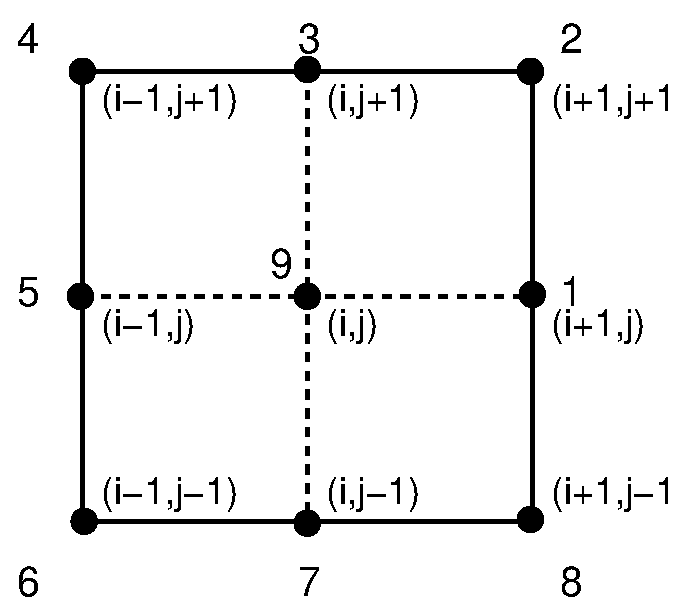
\includegraphics[scale=0.5]{./tex_plot/stencil.eps}
  \caption{Geometry for the 9 point stencil}
   \label{fig:stencil}
\end{figure}
%
The values at half grid points e.g. $(i+\frac{1}{2},j)$ are determined
by averaging the values of the adjacent grid points, e.g.
%
\begin{equation}
 \Sigma_{\phi \phi}^T(i+\frac{1}{2},j) = \frac{1}{2}
   \bigl[ \Sigma_{\phi \phi}^T(i+1,j) +  \Sigma_{\phi \phi}^T(i,j) \bigr]
\end{equation}
%
Accordingly, the values at $(i-\frac{1}{2},j)$, $(i,j+\frac{1}{2})$ and
$(i,j-\frac{1}{2})$ can be calculated. The difference at half points
in latitude and longitude e.g.  $(i+\frac{1}{2},j+\frac{1}{2})$
is also resolved by averaging the values of the adjacent grid 
points which leads to e.g.
%
\begin{equation}
\begin{split}
 &\Phi(i+\frac{1}{2},j+\frac{1}{2}) - \Phi(i+\frac{1}{2},j-\frac{1}{2}) =  \\
 &  \frac{1}{4}
   \bigl[ \Phi(i+1,j+1) -\Phi(i+1,j-1) + \Phi(i,j+1)- \Phi(i,j-1) \bigr]
\end{split}
\end{equation}
%
Accordingly, $\Phi(i-\frac{1}{2},j+\frac{1}{2}) - \Phi(i-\frac{1}{2},j-\frac{1}{2})$,
$\Phi(i+\frac{1}{2},j+\frac{1}{2}) - \Phi(i-\frac{1}{2},j+\frac{1}{2})$ and
$\Phi(i+\frac{1}{2},j-\frac{1}{2}) - \Phi(i-\frac{1}{2},j-\frac{1}{2})$ are discretized.
The resulting contributions from the conductance terms to the nine 
point stencil in figure \ref{fig:stencil}
are summarized in table \ref{tab:stencil}. 
Therein, we are using the abbreviations $A, B, C, D$  from equations
(\ref{eq:sig_dif1})--(\ref{eq:sig_dif4}) for the conductance quantities.
%
\begin{sidewaystable}
%\begin{table}
\begin{tabular}{|p{0.5cm} ||c|c|c|c|c|c|} \hline
 node  & $ A=\frac{\Sigma_{\phi \phi}^T}{\Delta \phi^2 cos \lambda_0}$
       & $B= \frac{\Sigma_{\lambda \lambda}^T(0) cos \lambda_0}{\Delta \lambda_0^2}$
       & $C= \frac{\Sigma_{\phi \lambda}^T(0)}{4\Delta \lambda_0 \Delta \phi }$
       & $D= \frac{\Sigma_{\lambda \phi}^T(0)}{4 \Delta \lambda_0 \Delta \phi}$  \\ \hline \hline
%
1  &$A(i+\frac{1}{2},j)$ & - & - &$D(i,j+\frac{1}{2})- D(i,j-\frac{1}{2})$    \\ 
2  &-&- &$C(i+\frac{1}{2},j) $ &$D(i,j+\frac{1}{2})$ \\ 
3  &-& $B(i,j+\frac{1}{2}) $&$C(i+\frac{1}{2},j)-C(i-\frac{1}{2},j)$ & -     \\ 
4  &-& -&$ -C(i-\frac{1}{2},j)$ &$ -D(i,j+\frac{1}{2})$      \\ 
5  &$A(i-\frac{1}{2},j)$&- & - & $-D(i,j+\frac{1}{2})+ D(i,j-\frac{1}{2})$   \\ 
6  &-& -&$ C(i-\frac{1}{2},j)$ &$D(i,j-\frac{1}{2})$ \\ 
7  &-&$B(i,j-\frac{1}{2})$ &$ -C(i+\frac{1}{2},j)+C(i-\frac{1}{2},j)$ & -    \\ 
8  &-& -&$ -C(i+\frac{1}{2},j)$ &$-D(i,j-\frac{1}{2})$       \\ 
9  &$-A(i+\frac{1}{2},j)-A(i-\frac{1}{2},j)$&$-B(i,j+\frac{1}{2})-B(i,j-\frac{1}{2})$ & - & -\\ \hline
%
\end{tabular}
\caption{Contributions from conductance terms to nine point stencil using central differencing
for all terms (see \src{subroutine cnm} and \src{subroutine cnmmod})}
\label{tab:stencil}
%\end{table}
\end{sidewaystable} 
%
%
\paragraph{Upwinding}
In the following the contributions to the stencil
are denotes by the variable c, e.g. at node 9 the coefficient would be c(i,j).
The stability is not preserved if the stencil coefficient of adjacent points 
of c(i,j) are changing sign e.g. $c(i+1,j)c(i-1,j) <0$ or
$c(i,j+1)c(i,j-1) <0$.
To avoid instabilities the diagonal dominance of the coefficient matrix
has to be preserved. This can be done by using upwinding methods 
depending on the orientation of the flux (i.e. the sign of the
stencil coefficients).   The derivatives with respect to e.g. $\lambda_0$ for the central
differencing is
%
\begin{equation}
 \frac{d\Phi(i+\frac{1}{2},j)}{d \lambda_0} = \frac{1}{\Delta \lambda_0} \bigl[ 
    \Phi(i+\frac{1}{2},j+\frac{1}{2}) - \Phi(i+\frac{1}{2},j-\frac{1}{2})\bigr]
\end{equation}
%
and the upwinding leads to
%
\begin{align}
\begin{split}
 \frac{d\Phi(i+\frac{1}{2},j)}{d \lambda_0} &= \frac{1}{2} \bigl[ 
   \frac{d\Phi(i+1,j)}{d \lambda_0}+ \frac{d\Phi(i,j)}{d \lambda_0}\bigr] \\
   &=\frac{1}{2 } \bigl[ \frac{\Phi(i+1,j+1) - 
   \Phi(i+1,j-1)}{2\Delta \lambda_0} + \frac{\Phi(i,j+1)- \Phi(i,j)}{ \Delta \lambda_0}
   \bigr] \\
 \frac{d\Phi(i+\frac{1}{2},j)}{d \lambda_0} &= \frac{1}{2} \bigl[ 
   \frac{d\Phi(i+1,j)}{d \lambda_0}+ \frac{d\Phi(i,j)}{d \lambda_0}\bigr] \\
   &=\frac{1}{2 } \bigl[ \frac{\Phi(i+1,j+1) - 
   \Phi(i+1,j-1)}{2\Delta \lambda_0} + \frac{\Phi(i,j)- \Phi(i,j-1)}{ \Delta \lambda_0}
   \bigr]
\end{split}
\end{align}
%
and for the derivative with respect to longitude $\phi$ the upwinding results in
%
\begin{align}
\begin{split}
 \frac{d\Phi(i,j+\frac{1}{2})}{d \phi_0} =& \frac{1}{2} \bigl[ 
   \frac{d\Phi(i,j+1)}{d \phi_0}+ \frac{d\Phi(i,j)}{d \phi_0}\bigr] \\
   &= \frac{1}{2 } \bigl[ \frac{\Phi(i+1,j+1) - 
   \Phi(i-1,j+1)}{\Delta \phi_0} + \frac{\Phi(i+1,j)- \Phi(i,j)}{2 \Delta \phi_0}
   \bigr] \\
\frac{d\Phi(i,j+\frac{1}{2})}{d \phi_0} =& \frac{1}{2} \bigl[ 
   \frac{d\Phi(i,j+1)}{d \phi_0}+ \frac{d\Phi(i,j)}{d \phi_0}\bigr] \\
   &= \frac{1}{2 } \bigl[ \frac{\Phi(i+1,j+1) - 
   \Phi(i-1,j+1)}{2 \Delta \phi_0} + \frac{\Phi(i,j)- \Phi(i-1,j)}{ \Delta \phi_0}
   \bigr] 
\end{split}
\end{align}
%
The flux at the center of the stencil (i, j) is 
determined by the flux average of the two adjacent points in the corresponding
direction. Thus, the latitudinal flux at the center c(i,j) is $f_l= \frac{1}{2}
[c(i,j+1) +c(i,j-1) ]$  and the longitudinal flux is  $f_l= \frac{1}{2}
[c(i+1,j) +c(i-1,j) ]$. For positive flux $f_l >0$ the values in table
 \ref{tab:stencil_upp} are used and for negative  flux $f_l <0$ the
 modifications in table
 \ref{tab:stencil_upm} are applied. If the flux at the two adjacent points goes into the
 same direction $c(i+1,j)c(i-1,j)> 0$ or $c(i,j+1)c(i,j-1)> 0$ the 
 central differencing in table \ref{tab:stencil} is used.
%
\begin{table}[tb]
\begin{tabular}{|p{0.5cm} ||c|c|c|} \hline
 node  & $ C= \frac{\Sigma_{\phi \lambda}^T(0)}{4\Delta \lambda_0 \Delta \phi }$
       & $D= \frac{\Sigma_{\phi \lambda}^T(0)}{4 \Delta \lambda_0 \Delta \phi} $ \\ \hline \hline
%
1  & - &$2 D(i,j+\frac{1}{2})-2 D(i,j-\frac{1}{2})$	\\ 
3  &$2 C(i+\frac{1}{2},j)- 2 C(i-\frac{1}{2},j)$ & -	\\ 
5  & - &-	\\ 
7  & - &-	\\ 
9  &$-2 C(i+\frac{1}{2},j)+2 C(i+\frac{1}{2},j)$  &$-2 D(i,j+\frac{1}{2})+2 D(i,j-\frac{1}{2})$	\\ \hline
%
\end{tabular}
\caption{Modification to stencil due to upwinding with positive flux $f_l >0$
in \src{subroutine cnm} and \src{subroutine cnmmod}}
\label{tab:stencil_upp}
\end{table} 
%
\begin{table}[tb]
\begin{tabular}{|p{0.5cm} ||c|c|c|} \hline
 node  &$ C= \frac{\Sigma_{\phi \lambda}^T(0)}{4\Delta \lambda_0 \Delta \phi }$
       &$ D= \frac{\Sigma_{\phi \lambda}^T(0)}{4 \Delta \lambda_0 \Delta \phi}$  \\ \hline \hline
%
1  & - &-	\\ 
3  & - & -	\\ 
5  & - &$-2 D(i,j+\frac{1}{2})+2 D(i,j-\frac{1}{2})$	\\ 
7  &$-2 C(i+\frac{1}{2},j)+ 2 C(i-\frac{1}{2},j) $ &-	\\ 
9  & $2 C(i+\frac{1}{2},j)-2 C(i+\frac{1}{2},j)$   &$2 D(i,j+\frac{1}{2})-2 D(i,j-\frac{1}{2})$	\\ \hline
%
\end{tabular}
\caption{Modification to stencil due to upwinding with negative flux $f_l <0$
in \src{subroutine cnm} and \src{subroutine cnmmod}}
\label{tab:stencil_upm}
\end{table} 
%
\paragraph{Equatorial boundary}\label{finite_equator}
%
At the equator the coefficient stencil has to be modified to
take into account the boundary condition which was described 
in section \ref{fieldline_eq} eq. (\ref{eq:kmlamequator})--(\ref{eq:kqphi_mod}). 
The discrete modification to the right hand side was described in the
paragraph on page \pageref{page:finite_rhs} eq. (\ref{eq:rhs_eq1}) 
but the derivation will be explained in the
following together with the left hand side. \\
%
Including the
equatorial boundary condition eq. (\ref{eq:kmlamequator}) into the electrodynamo equation 
eq. (\ref{eq:edyn}) leads to eq. (\ref{eq:eldyn_eq}). The boundary condition can be rewritten
as
%
\begin{equation}
   \Sigma_{\lambda \phi}
    \frac{\partial \Phi}{\partial \phi_m} + 
   \Sigma_{\lambda \lambda} cos \lambda_m 
   \frac{\partial \Phi}{\partial |\lambda_m|} =  R_0 cos \lambda_m K_{m \lambda}^D
\end{equation}
%
and from which in discrete form follows that
%
\begin{equation}
 \begin{split}
   T_{\lambda}(i,j_{eq}+\frac{1}{2})+ T_{\lambda}(i,j_{eq}-\frac{1}{2}) 
   = & R_0 cos \lambda_0(j_{eq}+\frac{1}{2}) K_{m \lambda}^D(i,j_{eq}+\frac{1}{2}) + \\
     & R_0 cos \lambda_0(j_{eq}-\frac{1}{2}) K_{m \lambda}^D(i,j_{eq}-\frac{1}{2}) \label{eq:finite_eqbnd1}
 \end{split}
\end{equation}
%
with $T_{\lambda}$ defined in eq. (\ref{eq:tlambda}).
The electrodynamo equation at the equator (\ref{eq:eldyn_eq})) is discretizied by
%
\begin{equation}
   \begin{split}
    & \frac{1}{cos \lambda_0(j_{eq})} \biggl[ \frac{T_{\phi}(i+\frac{1}{2},j_{eq})-
     T_{\phi}(i-\frac{1}{2},j_{eq})}{\Delta \phi_0} + \frac{T_{\lambda}(i,j_{eq}+\frac{1}{2})-
     T_{\lambda}(i,j_{eq}-\frac{1}{2})}{\Delta \lambda_0} \biggr] = \\
   &  \frac{R_0}{cos \lambda_0 (j_{eq}) \Delta \phi_0} \biggl[  K_{m \phi}^{D, mod T}(i+\frac{1}{2},j_{eq}) - 
      K_{m \phi}^{D, mod T}(i-\frac{1}{2},j_{eq})
     \biggr] 
     + \\
   & \frac{R_0}{cos \lambda_0 (j_{eq}) \Delta \lambda_0}\biggl[K_{m \lambda }^{DT}(i,j_{eq}+\frac{1}{2}) 
    cos \lambda_0(j_{eq}+\frac{1}{2}) - K_{m \lambda }^{DT}(i,j_{eq}-\frac{1}{2}) 
    cos \lambda_0(j_{eq}-\frac{1}{2})   \biggr]\label{eq:finite_eqbnd2}
   \end{split}
\end{equation}
%
Inserting equation (\ref{eq:finite_eqbnd1}) into the electrodynamo equation 
(\ref{eq:finite_eqbnd2}) the values $K_{m \lambda }^{DT}(i,j_{eq}-\frac{1}{2})$
and $T_{\lambda}(i,j_{eq}-\frac{1}{2})$ are substituted by $K_{m \lambda }^{DT}(i,j_{eq}+\frac{1}{2})$
and $T_{\lambda}(i,j_{eq}+\frac{1}{2})$ which lead to
%
\begin{equation}
   \begin{split}
    & \frac{T_{\phi}(i+\frac{1}{2},j_{eq})-
     T_{\phi}(i-\frac{1}{2},j_{eq})}{\Delta \phi_0} + \frac{ 2 T_{\lambda}(i,j_{eq}+\frac{1}{2})
     }{\Delta \lambda_0}  = \\
   &  \frac{R_0}{ \Delta \phi_0} \biggl[  K_{m \phi}^{D, mod T}(i+\frac{1}{2},j_{eq}) - 
      K_{m \phi}^{D, mod T}(i-\frac{1}{2},j_{eq})
     \biggr] 
     + \\
   & \frac{R_0}{ \Delta \lambda_0}\biggl[2 K_{m \lambda }^{DT}(i,j_{eq}+\frac{1}{2}) 
    cos \lambda_0(j_{eq}+\frac{1}{2}) \biggr]\label{eq:finite_eqbnd3}
   \end{split}
\end{equation}
%
with $cos \lambda_0(j_{eq})=1$ and the value $T_{\phi} = \frac{\Sigma_{\phi \phi}^{mod T}(0)}{cos
   \lambda_0} \frac{\partial \Phi}{\partial \phi_0}$ at the equator.
Therefore the stencil has to be modified at the equator according to
table \ref{tab:stencil_eq} with $B(i,j-\frac{1}{2})=0$, $D(i,j-\frac{1}{2}) =0$
and no $\Sigma_{\phi \lambda}$ contributions. The coefficients for
A are not changing (see table \ref{tab:stencil}).
%
\begin{table}[tb]
\begin{tabular}{|p{0.5cm} ||c|c|c|c|c|} \hline
 node  & $A=\frac{\Sigma_{\phi \phi}^T}{\Delta \phi^2 cos \lambda_0}$
       & $B= \frac{\Sigma_{\lambda \lambda}^T(0) cos \lambda_0}{\Delta \lambda_0^2}$
       & $C= \frac{\Sigma_{\phi \lambda}^T(0)}{4\Delta \lambda_0 \Delta \phi }$
       & $D= \frac{\Sigma_{\phi \lambda}^T(0)}{4 \Delta \lambda_0 \Delta \phi}$ \\ \hline \hline
%
1  &$A(i+\frac{1}{2},j)$ &- &-&$D(i,j+\frac{1}{2})$	  \\ 
2  &- &- &-&$D(i,j+\frac{1}{2})$   \\ 
3  &- &$ B(i,j+\frac{1}{2})$&- & -	\\ 
4  &- &- &- &$-D(i,j+\frac{1}{2})$	 \\ 
5  &$A(i-\frac{1}{2},j)$ & - &-& $-D(i,j+\frac{1}{2})$  \\ 
6  &- &- &-& - \\ 
7  &- & - &-&  -	 \\ 
8  &- & -&-& -\\ 
9  &$-A(i+\frac{1}{2},j)-A(i-\frac{1}{2},j)$ &$-B(i,j+\frac{1}{2})$ &-&-    \\ \hline
%
\end{tabular}
\caption{Modification to stencil at the equator (see
 \src{subroutine cnm} or \src{subroutine cnmmod} )}
\label{tab:stencil_eq}
\end{table} 
\\

\paragraph{Coefficient stencil}
In table \ref{tab:c_level} the longitudinal and latitudinal dimensions 
of the 5 different grid levels are given. 
%
\begin{table}[tb]
\begin{tabular}{|p{1.5cm} ||c|c|c|c|c|} \hline
grid level   & variable $c^*$ & long.dimension& lat.dimension $nmlat^*$ & "points" of stencil\\ \hline \hline
%
0 &c0 & 81& 49& 10\\ 
1 &c1 & 41& 25& 9 \\ 
2 &c2 & 21& 13& 9 \\ 
3 &c3 & 11&  7& 9 \\ 
4 &c4 & 6 &  4& 9 \\ \hline
%
\end{tabular}
\caption{Coefficient matrix name and dimensions at the different grid levels}
\label{tab:c_level}
\end{table} 
%
On the finest grid level the right hand side is stored in $c0(:,:,10)$.
Therefore the dimension is 10 instead of 9, which is the size at all other grid
levels. At the pole ($j=nmlat^*$) the off diagonal terms are set to zero and the diagonal
terms to one $c^*(i,nmlat^*,9)=1$ in \texttt{subroutine edges} with $(\cdot)^*$ denoting the different grid
levels. The right hand side is set to one at the
pole  $c0(i,nmlat,10)=1$. The left hand side $lhs$ is finally divided 
by $cos \lambda_0$ in \texttt{subroutine divide}.

%
\section{Solving for the electric potential} \label{cap:solve}
%
In TIEGCM a multigrid solver is used which was developed by
J. Adams. The source code and information can be found at
http://www.scd.ucar.edu\-/css\-/software\-/mudpack/. In the original mudpack solver 
the finite differencing and the setting of all the boundary conditions
are part of solver package. For TIEGCM the stencil and the boundary
conditions  are
already set up in the TIEGCM code, and therefore the multigrid
solver was modified accordingly. We have three different solver
options in TIEGCM which are all based on the mudpack multigrid package.
%
\begin{itemize}
  \item \flags{isolve=0} multigrid solver \src{mudcr2} (see section \ref{cap:mudsol})
  \item \flags{isolve=1} multigrid solver \src{muhcr2} as direct solver (see section 
         \ref{cap:directsol})
  \item \flags{isolve=2} modified multigrid solver \src{mudcr2} (see section 
         \ref{cap:modmudsol})
\end{itemize}
%
%
\subsection{Multigrid solver \texttt{mudcr2}}\label{cap:mudsol}
%
The \texttt{subroutine mud2cr} attempts to compute
the second-order difference approximation to a two-dimensional
linear nonseparable elliptic partial differential equation with cross
derivative terms on a rectangle.  The approximation is generated on a
uniform grid covering the rectangle. The parameters used for the multigrid solver 
in TIEGCM are the following:
%
\begin{itemize}
  \item \flags{intl=0}: this is an input to the subroutine and is zero for the initial
           call to \texttt{mud2cr} to check for errors. After the initial 
	   call of \texttt{mud2cr} \flags{intl=1} will be set and the PDE is solved.
  \item boundary conditions: with x being the longitudinal direction and y the
          latitudinal one from the equator to the pole.
  \begin{itemize}  
      \item \flags{nxa =0 }: flags boundary conditions on the edge x=xa. nxa = 0
    		means the boundary condition is periodic in x on [xa,xb].
      \item \flags{nxb =0}: flags boundary conditions on the edge x=xb.  nxb = 0
    		means the boundary condition is periodic in x on [xa,xb].
      \item \flags{nyc =2}: flags boundary conditions on the edge y=yc (equator). nyc = 2 means
    		that there are mixed derivative boundary conditions at y=yc.
      \item \flags{nyd =1}: flags boundary conditions on the edge y=yd (pole). nyd=1 means
      that the boundary condition is specified and input thru the variable \src{phi}.
  \end{itemize}
  \item  defining the number
    	    of grid points in x (longitude) and y (latitude) direction
  \begin{itemize} 
    \item \flags{ixp = 5}: ixp+1
  	    is the number of points on the coarsest x grid visited during
  	    multigrid cycling.
    \item \flags{jyq = 3}: jyq+1 
  	    is the number of points on the coarsest y grid visited during
  	    multigrid cycling.
    \item \flags{iex = 5}: integer exponent of 2 used in defining the number
    	    of grid points in the x direction 
    \item \flags{jey = 5}: integer exponent of 2 used in defining the number
    	    of grid points in the y direction 
    \item \flags{nx}: number of equally spaced grid points in the interval [xa,xb]
    		$ nx = ixp \; 2^{iex-1} + 1$
    \item \flags{ny}: number of equally spaced grid points in the interval [yc,yd]
    		$ ny = jyq \; 2^{jey-1} + 1$
  \end{itemize}
  \item \flags{iguess = 0:} no initial guess is used  forcing full multigrid cycling
  \item \flags{tolmax = 0.01}: 
        tolmax is the maximum relative error tolerance
	  used to terminate the relaxation iterations. Assume $\Phi_1$
	  and $\Phi_2$ are the last two computed approximations at 
	  the finest grid level. If we define \\
	     $ \Phi_{diff} = max(|\Phi_2(i,j)-\Phi_1(i,j)|) \quad \text{for all} \quad i,j$
	  and \\
	      $ \Phi_{max} = max(|\Phi_2(i,j)|) \quad \text{for all} \quad i,j $
	  then convergence is considered to have occurred if and only if
	      $ \frac{\Phi_{diff}}{\Phi_{max}} < tolmax  $
  \item \flags{maxcy = 150}: if $tolmax > 0.0$
	  is input, which means error control is used, then maxcy is the limit on the number
	  of cycles between the finest and coarsest grid levels. 
	  When the multigrid iteration is working
          correctly only a few cycles are required for convergence.
  \item \flags{method = 3}: method of relaxation. If neither fx (the longitudinal
       second order derivative $\Sigma_{\phi \phi}/ \Delta \phi^2$) or fy (the latitudinal
       second order derivative $\Sigma_{\lambda \lambda}/ \Delta \lambda_0^2$) dominates 
       over the solution region and they
       both vary considerably choose method = 3, which uses line 
       relaxation in both the x and y direction
  \item \flags{nwork}: length of work array \\
        $length = [7(nx+2)(ny+2)+4(11+isx+jsy)nx*ny]/3$
  \item \flags{mgopt}: multigrid options the default values 
     (2,2,1,3) in the vector \src{mgopt} were chosen for
     robustness.
     \begin{itemize}
         \item \flags{mgopt(1) = 2}: w cycling 
         \item \flags{mgopt(2) = 2}: the number of pre--relaxation 
	   sweeps executed before the
           residual is restricted and cycling is invoked at the next
           coarser grid level
         \item \flags{mgopt(3) = 1}: the number of post--relaxation sweeps executed after the cycling
           has been invoked at the next coarser grid level and the residual
           correction has been transferred back
         \item \flags{mgopt(4) = 3}: multicubic prolongation 
	      (interpolation) is used to
              transfer residual corrections and the PDE approximation
              from the coarse to the fine grid within full multigrid cycling.
     \end{itemize}
  \item output \flags{$\Phi$}: solution of PDE which is the electric potential
  \item output \flags{ierror}: indicates invalid input arguments when
          returned positive and nonfatal warnings when returned
          negative.
%
\end{itemize}
%
If no convergence is reached with this version of the multigrid solver the direct
solver described in section \ref{cap:directsol} is used.
%
\subsection{Multigrid solver \src{muhcr2} as direct solver}\label{cap:directsol}
%
This solver which is in \texttt{subroutine muh2cr} is originally a hybrid 
multigrid/direct method which approximates the
same 2-d nonseparable elliptic PDE as the mudpack solver \src{mud2cr}.
Using a direct method combines the efficiency of multigrid iteration 
with the certainty of
a direct method.  The basic algorithm is modified by using banded
Gaussian elimination in place of relaxation whenever the coarsest
subgrid is encountered within the multigrid cycling.
The solver becomes a full direct method if grid size arguments are chosen
so that the coarsest and finest grids coincide, i.e.  choosing iex=jey=1
and ixp=nx-1, jyq=ny-1. This will set the Gaussian elimination
on the finest grid.  In this case, \texttt{subroutine muh2cr} produces a 
direct solution
to the same nonseparable elliptic PDE. In TIEGCM we are using the
solver \src{muhcr2} only as a direct solver.
%
\subsection{Modified multigrid solver \src{mudcr2}}\label{cap:modmudsol}
%
This solver is the same as the solver in section \ref{cap:mudsol} only with the
exception that the residual is calculated with the coefficient
stencil without upwinding (see section \ref{chap:finitediff}). Therefore 
the solution converges toward 
the solution of the direct solver using the 
coefficient stencil without the upwinding method.
In general upwinding introduces unwanted numerical dissipation. 
The unmodified
coefficient stencil is stored in the array \src{cofum}. 
In comparison with the solver in
section \ref{cap:mudsol} the number of relaxation
steps has to be increased to get convergence.
%
\begin{itemize}
    \item \flags{mgopt(2) = 3}: the number of pre--relaxation 
      sweeps executed before the
      residual is restricted and cycling is invoked at the next
      coarser grid level
    \item \flags{mgopt(3) = 2}: the number of post--relaxation sweeps executed after cycling
      has been invoked at the next coarser grid level and the residual
      correction has been transferred back
\end{itemize}
%
All the other parameters remain the same and can be found in section 
\ref{cap:mudsol}.
If no convergence is reached with this multigrid solver the direct
solver described in section \ref{cap:directsol} is called.
%

%
%
\section{Electric Field}
%
In \src{subroutine threed} the two and three dimensional 
electric field and the three dimensional electric potential 
is calculated from the two dimensional electric
potential $\Phi$. The components of the electric field $E_{d1}$ and $E_{d2}$
which are in more-or-less magnetic eastward and downward/equatorward direction are
determined by
%
\begin{align}
   E_{d1} &= - \frac{1}{R_0 cos \lambda_m}\frac{\partial \Phi}{\partial \phi_m} \\
   E_{d2} &= \frac{1}{R_0 sin I_m}\frac{\partial \Phi}{\partial \lambda_m}
\end{align}
%
In the code the equally spaced latitudinal grid point
distribution $\lambda_0$ in $\lambda_m^*$ is used to calculate the derivatives. Therefore 
the mapping factors from the irregular latitudinal spaced 
grid $\lambda_m^*$ to $\lambda_0$ have to be taken into account. 
Including these factors the discrete derivatives are
%
\begin{align}
   E_{d1}(i,j) &= - \frac{1}{R_0}\frac{cos \lambda_0(j)}{cos \lambda_m^*(j)}
           \frac{ \Phi(i-1,j) -\Phi(i+1,j) }{2 cos \lambda_0(j) \Delta \phi_m} \\
   E_{d2}(i,j) &= \frac{1}{R_0}\frac{\partial \lambda_0(j)}{|sin I_m(j)|
               \partial \lambda_m^*(j)}
            \frac{\Phi(i,j-1) -\Phi(i,j+1)}{2 \Delta \lambda_0}
\end{align}
%
The polar values are averaged over the four surrounding points. At the equator a
second order polynomial of the electric potential is fitted through the adjacent points
and thus the derivative of the polynomial at the equator is determined. \\

The three dimensional electric potential and electric field is calculated
assuming that the dipolar magnetic field lines are equipotential. At each grid 
point $(\phi(i),\lambda_m^*(j),h(k))$
the foot point of the magnetic field line going through this grid point is
determined. Having found the foot point of the field line at height $h_0$
the values, i.e. electric potential and electric field, 
at this point can be determined by a two dimensional interpolation of
the surrounding points. The polar values are determined by longitudinal 
averaging all the polar values.

%
\section{Additional features}
%
%
\subsection{Magnetic perturbations}
%
The magnetic perturbation from a TIEGCM model run can be determined
by using the postprocessor program \src{MagIon}. The program is available
upon request together a \src{MagIon} user guide, a model description
is in preparation. The global magnetic perturbations
at the ground and above the ionosphere at low orbiting satellite heights
can be determined, 
or what a magnetometer would measure at the ground. 
For details about the calculation and the
necessary assumption we refer to  \cite{rich74} and the 
\src{MagIon} user guide. \\

%
To calculate the magnetic perturbation the radial component of the field-aligned current
$J_{qr}$ and the height--integrated current densities $K_{m \phi}$
and $K_{m \lambda}$ have to be known. In addition, if the influence of 
gravity and plasma
pressure gradient driven current
should be included the height dependent $K_{m \phi}^{int}$
have to be determined with and without the current driven by gravity and plasma
pressure gradient. The calculation of these currents
is not the default in the TIEGCM source code, thus the flag  \flags{icalkqlam == 1} 
in the \src{module dynamo} has to be set. In the following the
calculation of the different currents $J_{qr}$, $K_{q \phi}$ and $K_{q \lambda}$, 
which can be found in the file \src{current.F}, is described. 
%
\subsubsection{Field--aligned current $J_{qr}$}\label{chap:jqr}
% 
The field--aligned current can be determined from the electrodynamo
equation (\ref{eq:edyn}) without the assumption of symmetrical
hemispheres which leads to 
%
\begin{equation}
 \begin{split}
  & \frac{\partial}{\partial \phi_m} \bigl( \frac{\Sigma_{\phi \phi}}{cos
   \lambda_m} \frac{\partial \Phi}{\partial \phi_m} + 
   \Sigma_{\phi \lambda} \frac{\partial \Phi}{\partial |\lambda_m|} \bigr) +
   \frac{\partial}{\partial | \lambda_m |} \bigl( \Sigma_{\lambda \phi}
    \frac{\partial \Phi}{\partial \phi_m} + 
   \Sigma_{\lambda \lambda} cos \lambda_m 
   \frac{\partial \Phi}{\partial |\lambda_m|} \bigr) \\
  &  =
   R \frac{\partial K_{m \phi}^{D}}{\partial \phi_m} +  
   R \frac{\partial K_{m \lambda cos \lambda_m }^{D}}{\partial | \lambda_m |} +
   R^2 cos \lambda_m J_{mr}
    \label{eq:edyn_wosym}
  \end{split}
\end{equation}
%
Note that compared to the electrodynamo equation (\ref{eq:edyn}) the
conductances and the wind driven current are different in the northern and
southern hemisphere denoted by e.g. $\Sigma_{\phi \phi}$ instead of 
$\Sigma_{\phi \phi}^T$. Therefore we determine the finite difference coefficient 
stencil for both
hemispheres instead of only one as described in section \ref{chap:finitediff} on
page \pageref{page:diff_lhs}. The set up of the finite difference stencil  
is analog to the one for only one
hemisphere. The  \src{subroutine nosocoef} sets up the
coefficient stencil for both hemisphere and also saves the wind driven current.
The  \src{subroutine nosocoef} is called shortly after the field line
integrations i.e. before the conductances and wind driven currents are added
together from the two hemispheres (see table \ref{tab:transf_quantities}). 
The conductances are prepared for the finite differencing
and represent 
% 
\begin{align}
A=& \frac{\Sigma_{\phi \phi}(0)}{cos\lambda_0  \Delta \phi^2 }	   \rightarrow  nszigm11\label{eq:nssig_dif1}\\
B=& \frac{\Sigma_{\lambda \lambda}^(0) cos \lambda_0}{\Delta \lambda_0^2} \rightarrow  nszigm22\label{eq:nssig_dif2} \\
C=& \frac{\Sigma_{\phi \lambda}(0)}{4\Delta \lambda_0 \Delta \phi }    \rightarrow  nszigmc \label{eq:nssig_dif3} \\
D=& \frac{\Sigma_{\phi \lambda}(0)}{4 \Delta \lambda_0 \Delta \phi}    \rightarrow  nszigm2 \label{eq:nssig_dif4} 
\end{align}
%
The set up of the stencil is analog to section \ref{chap:finitediff}
see table \ref{tab:stencil} and \ref{tab:stencil_eq} with A, B, C and D
from the definitions above eq. (\ref{eq:nssig_dif1})--(\ref{eq:nssig_dif4}). \\

The calling tree is 
%
\begin{verbatim}
...
call nsstencil
   call nscnm
...
\end{verbatim}
%
Note that the stencil is only calculated on the finest grid. In addition
no  upwinding method to preserve the diagonal dominance is used  
since the finite difference stencil is not used for solving. The numbering
 of the nine node stencil for the
southern hemisphere is the same as for the northern hemisphere, which is illustrated in 
 figure \ref{fig:nsstencil} for both hemispheres. This means that e.g. points 6'', 7'' and 8'' 
in the southern hemisphere are toward the poles and not toward the equator as for the northern hemisphere
points 6, 7 and 8.
This switch of the nodes 6, 7, 8 with 4, 3, 2 is reflected in the set up
of the stencil in the southern hemisphere done in \src{subroutine nscnm}.
The result is stored in the array \src{nscoef}. The wind driven currents
of the right hand side are treated in the same way as in the dynamo
equation in section  \ref{chap:finitediff} on page \pageref{page:finite_rhs}.
The right hand side is saved in the array \src{nsrhs}.
 \\
 
%
\begin{figure}
  \centering
  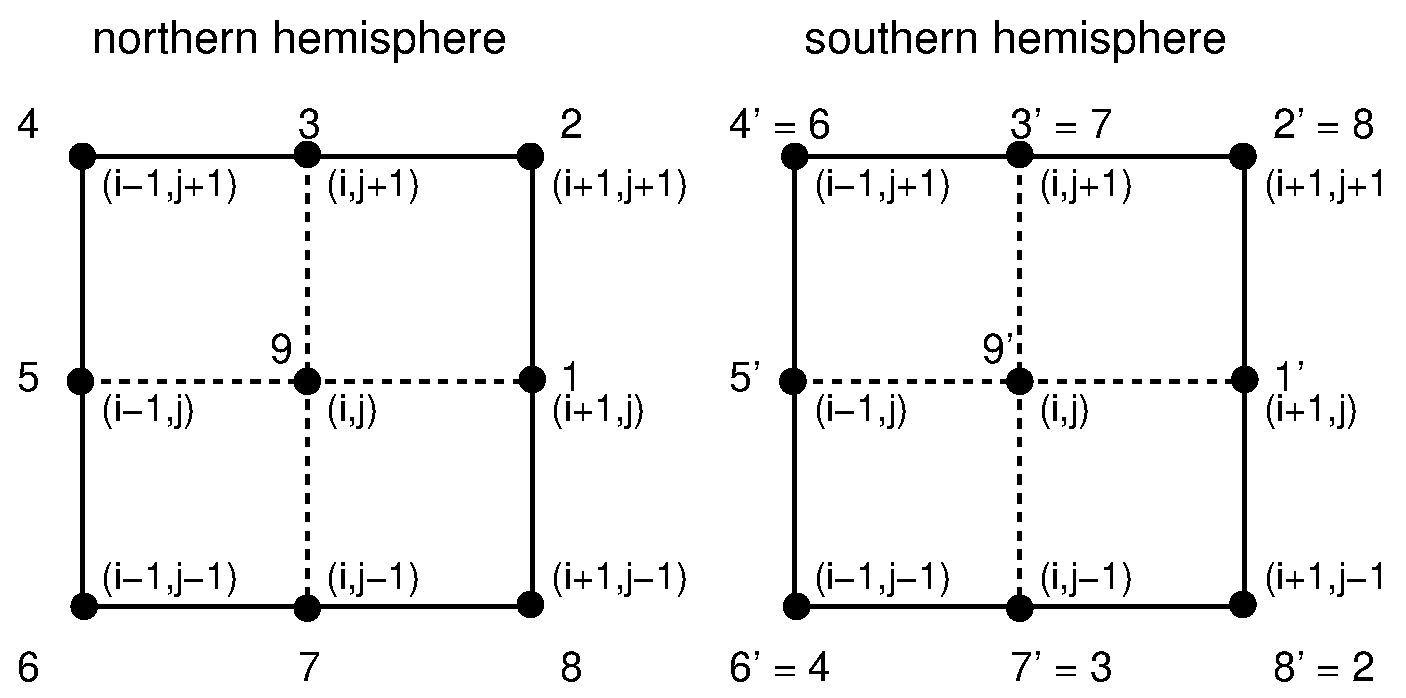
\includegraphics[scale=0.5]{./tex_plot/ns_stencil.eps}
  \caption{Geometry for the 9 point stencil in the northern and southern hemisphere}
   \label{fig:nsstencil}
\end{figure}
%

Having set up the finite difference coefficient matrix $\bar{\mathbf{C}}$ of the 
left hand side, as described
in the previous paragraph, and determined the wind driven current of the right
hand side vector $\mathbf{rhs}$ we can insert the 
calculated electric potential vector $\mathbf{\Phi}$ 
into equation
(\ref{eq:edyn_wosym}) to solve for the field aligned current vector $\mathbf{J}_{mr}$.
%
\begin{equation}
   R_0^2 \frac{cos \lambda_m}{cos \lambda_0}
  \frac{\partial \lambda_0}{\partial \lambda_m^*} J_{mr} = \bar{C} \Phi - \text{rhs} \label{eq:jmr_solve}
\end{equation}
%
Note that the whole electrodynamo equation was multiplied by
$\frac{1}{cos \lambda_0}\frac{\partial \lambda_0}{\partial \lambda_m^*}$ as mentioned 
on page \pageref{page:electro_multi}. The current calculation is done
in \src{subroutine nosocrrt}. For the polar values the average values at
adjacent latitudinal point are extrapolated by
%
\begin{align}
  J_{mr} (j_{pole})= & \frac{1}{8 \text{nmlon}} \bigl[ 
     9\sum_{i=1}^{nmlon} {J}_{mr} (i,j_{pole} \mp 1)
    - \sum_{i=1}^{nmlon} {J}_{mr} (i,j_{pole} \mp 2)\bigr] 
\end{align}
%
with $nmlon$ the number of longitudes and $j_{pole}$ the latitudinal index at
the north / south pole and the $\mp$ sign referring to the poles
respectively. 
Close to the magnetic equator there is no distinct allocation of the
current to either the height integrated current density $K_{m \lambda}$
or the field--aligned current $J_{mr}$ since the magnetic field lines are
almost horizontal in this region. Therefore the allocation to either one of 
the two currents $K_{m \lambda}$ and $J_{mr}$ depends strongly on the 
reference height $h_0$. Raising the reference height will shift the current 
from the field line to the ionospheric current sheet $K_{m \lambda}$. The 
exact distribution of the current at the equator can be neglected for the
calculation of the magnetic perturbations. Therefore we linearly interpolate 
the field--aligned current between $\pm 12^o$ latitude.
%
\begin{align}
  J_{mr} (j)= \frac{J_{mr}(\lambda_m^{max}) J_{mr}(\lambda_m^{min}) }
  {\lambda_m^{max} - \lambda_m^{min}} (\lambda_m-\lambda_m^{min}) 
  + J_{mr} (\lambda_m^{min}) & \\
    \quad \text{for} \quad \lambda_m^{min} \leq \lambda_m \leq \lambda_m^{max} &
\end{align}
% 
with $\lambda_m^{min} = -12^o$ and $\lambda_m^{max} = 12^o$. 
Due to the linear interpolation at each latitude
higher frequency modes are introduced which are smoothed by a weighted
average in longitude.
%
\begin{align}
  J_{mr} (j)= \frac{1}{5} [J_{mr}(i+1,j) + 3 J_{mr}(i,j) + J_{mr}(i-1,j)  ]
\end{align}
% 
Since the field--aligned
current $J_{mr}$ is used to calculate the ionospheric equator-- / 
downward current sheet contribution
 $K_{m \lambda}$ the total current system
 is adjusted automatically to satisfy that it is divergence free.
 
%
\subsubsection{Eastward current $J_{e1}$ and height integrated current densities
 $K_{q\phi}$, $K_{q\lambda}$}
% 
To calculate the eastward height integrated current density $K_{q \phi}$, see also
eq. (7.4) in \cite{rich95},
%
\begin{align}
  K_{q \phi} = \int_{h_l}^{h_u} \bigl(\frac{R_E+h}{R_0}\bigr)^{5/2} \frac{J_{e1}}{F} dh
  \label{eq:kmphi_1}
\end{align}
% 
the eastward current $J_{e1}$ has to be known. The eastward current $J_{e1}$ is
determined by, see also
eq. (5.7) in \cite{rich95},
%
\begin{align}
  \frac{J_{e1}}{D} = \sigma_P \frac{d_1^2}{D}(E_{d1} + u_{e2}B_{e3}) + 
      (\sigma_P \frac{\mathbf{d}_1 \cdot \mathbf{d}_2}{D} - \sigma_H)
      (E_{d2} - u_{e1}B_{e3}) + \text{fac} \frac{J_{e1}^{p,g}}{D}
\end{align}
% 
The downward--/ equatorward current component $J_{e2}$ is only calculated for postprocessing
reasons.
%
\begin{align}
  \frac{J_{e2}}{D} = \sigma_P \frac{d_2^2}{D}(E_{d2} - u_{e1}B_{e3}) + 
      (\sigma_P \frac{\mathbf{d}_1 \cdot \mathbf{d}_2}{D} + \sigma_H)
      (E_{d1} + u_{e2}B_{e3}) + \text{fac} \frac{J_{e2}^{p,g}}{D}
\end{align}
%
with $\text{fac}=10^4$ being the conversion factor from $\frac{1}{cm^2}$ to $\frac{1}{m^2}$. 
The current components are computed on the half pressure levels. The input
quantities $\sigma_H$, $\sigma_P$, $\frac{d_1^2}{D}$, 
$\frac{\mathbf{d}_1 \cdot \mathbf{d}_2}{D}$, $u_{e1}$, $u_{e2}$ and $B_{e3}$ are
all stored at half pressure levels. Only the electric field $E_{d1}$ and $E_{d2}$
are at full pressure levels and have to be converted to half levels by
%
\begin{align}
   E_{d1}(k') = \frac{1}{2} (E_{d1}(k) + E_{d1}(k+1) )
\end{align}
% 
with k' denoting the half pressure level index $k' = k+ \frac{1}{2}$. We assume that
$\frac{d_2^2}{D} =1$ everywhere which is approximately true. In addition to this
simplification the height variation of the magnetic field component $B_{e3}$
is neglected. The current contribution due to plasma pressure gradient and gravity 
$J_{e1}^{p,g}$ is
%
\begin{align}
  \frac{J_{e1}^{p,g}}{D} = \frac{\mathbf{J}_{p}\cdot \mathbf{d}_1 + 
          \mathbf{J}_{g}\cdot \mathbf{d}_1}{D}  
\end{align}
% 
with $\mathbf{J}_{p}$ determined in section \ref{subsec:ppres_current}  by
eq. (\ref{eq:j_p}) and the gravity term  $\mathbf{J}_{g}$ in section 
\ref{subsec:grav_current} by eq. (\ref{eq:j_g}). The gravity and plasma pressure 
gradient current is calculated in \src{subroutine magpres\_grav} on the
geographic grid and is mapped afterward to the geomagnetic grid. Both terms $\mathbf{J}_{p}$
 and $\mathbf{J}_{g}$ are stored at half pressure levels. \\
 
Once the eastward current $J_{e1}$ is determined the height integrated
eastward current density $K_{m \phi}$ can be calculated by using eq. (\ref{eq:kmphi_1})
with the dipole filed quantity
 $F$ quantity, see also eq. (6.9) in \cite{rich95},
%
\begin{align}
  F = \frac{sin \lambda_m}{sin \lambda_q}\frac{sin I}{sin I_m}\bigl(\frac{R_E+h}{R_0}\bigr)^3 D
  \label{eq:kqphi_f} 
\end{align}
% 
Inserting eq. (\ref{eq:kqphi_f}) into eq. (\ref{eq:kmphi_1}) leads to
%
\begin{align}
 K_{q \phi} = \int_{h_l}^{h_u} \frac{J_{e1}}{D} 
 \frac{sin \lambda_q}{sin \lambda_m}\frac{sin I_m}{sin I}\bigl(\frac{R_0}{R_E+h}\bigr)^{1/2} dh
  \label{eq:kqphi_insert} 
\end{align}
% 
which is calculated at full pressure levels. The height integrated current densities are
calculated assuming a dipole field which is indicated by the index $(\cdot)_q$ of
$K_{q \phi}$. Therefore the height integration is done in height rather than along
the field line. The difference between height and field line integration at mid--
and high latitude is small since the field lines are almost vertical through
the ionospheric current sheet. 
The dipole latitude $\lambda_q$ in 
eq. (\ref{eq:kqphi_insert}) is
%
\begin{align}
 sin \lambda_q (h) = sin \lambda_m (h_0)
\end{align}
% 
We assume dipolar field lines such that $\lambda_m (h)$ can be computed by
%
\begin{align}
 cos^2 \lambda_m (h) = \frac{R_0}{R} cos^2 \lambda_q
\end{align}
% 
The sinus of the inclination angle $I_m$ is determined by
%
\begin{align}
  sin I_m = \frac{2 sin \lambda_m(h_0)}{\sqrt{1 + 3 sin^2 \lambda_m(h_0)}}
\end{align}
% 
and the sinus of the angle $I$ by
%
\begin{align}
  sin I = \frac{B_z}{|B_0|}
\end{align}
% 
with $|B_0|$ the magnitude of the geomagnetic field and $B_z$
the downward component. Note that we assume that both quantities vary
in the same way in height and therefore no height variation is taken
into account. The equatorial values of $ sin I $ and $sin \lambda_q$
are taken from the adjacent grid point in latitude. The height integral
is the sum over all height levels with
%
\begin{align}
  K_{q \phi} = \sum_{k=-2}^{\text{mlev}} S(k') 
    J_{e1}(k') dh(k) \label{eq:kqphi_total}
\end{align}
% 
with $J_{e1}(k')$ the eastward current at the half pressure level between k and k+1.
The term S denotes $\frac{sin \lambda_q}{sin \lambda_m}\frac{sin I}{sin I_m}
(\frac{R_0}{R_E+h})^{1/2}$ which is known at the full level e.g. k and k+1
and therefore has to be interpolated to the half pressure level. 
The discrete height
$dh$ is determined by $dh = \frac{1}{100} [z(k+1) - z(k)]$ in [m]. \\
%
For the
calculation of the magnetic perturbations due to plasma pressure gradient and
gravity driven current, the height distribution of the eastward current density denoted by 
$K_{m \phi}^{int}$ has to be known. The previous assumption that most of the current is
flowing in a thin current shell is not valid anymore since the current due to
gravity and plasma pressure gradient is flowing in the E-- and F--region.
Therefore the height dependent current density at pressure level $k^*$ is
calculated by
%
\begin{align}
  K_{m \phi}^{\text{int}}(k^*) = \sum_{k=-2}^{k^*} S(k')
    J_{e1}(k') dh(k)\label{eq:kqphi_int}
\end{align}
% 

%
Once the height integrated eastward current density $K_{q \phi}$ and the radial
component of the field aligned current $J_{mr}$ are determined by equations 
(\ref{eq:jmr_solve}) and (\ref{eq:kqphi_total}) the height integrated northward
current density $K_{q \lambda}$ can be calculated such that the current system is
divergence free
%
\begin{align}
  J_{mr} = \frac{-1}{R cos \lambda_q} \bigl[ 
    \frac{\partial K_{q \phi}}{\partial \phi_q} + 
    \frac{\partial (K_{q \lambda} cos \lambda_q)}{\partial \lambda_q}  
    \bigr]\label{eq:jmr_div}
\end{align}
% 
Solving eq. (\ref{eq:jmr_div}) for the the height integrated northward 
current density $K_{q \lambda}$ leads to
%
\begin{align}
  K_{q \lambda} (\phi_q,\lambda_q^*)= - \frac{1}{cos \lambda_q^*} \int_{-\frac{\Pi}{2}}^{\lambda_q^*}
   \bigl[ J_{mr} R cos \lambda_q + \frac{\partial K_{q \phi}}{\partial \phi_q} 
   \bigr] d \lambda_q\label{eq:kmlambda}
\end{align}
% 
The derivative $\frac{\partial K_{q \phi}}{\partial \phi_q}$ is approximated by
central differencing
%
\begin{align}
   \frac{d K_{q \phi}(i,j)}{d \phi_q} = \frac{K_{q \phi}(i + \frac{1}{2},j) - 
   K_{q \phi}(i - \frac{1}{2},j)}{2 \Delta \phi_q} 
   \label{eq:deriv_kqphi}
\end{align}
%
with i being the longitudinal index and $i + \frac{1}{2}$ denoting the average
between the grid points i and i+1. We substitute the following term for
simplicity 
%
\begin{align}
   T(i,j) =  J_{mr}(i,j) R cos \lambda_q(j) + \frac{d K_{q \phi}(i,j)}{d \phi_q}
   \label{eq:kqlam_simpl}
\end{align}
%
into equation (\ref{eq:kmlambda}). The integration is done over the
southern and northern hemisphere separately since the total current in
both hemispheres has to cancel. 
%
\begin{align}
   S^{SH}(i,j^*) &= - \sum_{j=2}^{j^*} T(i,j-\frac{1}{2})[\lambda_j - \lambda_{j-1}]
    \quad \frac{nmlat+1}{2} \ge j^* > 2 \label{eq:kqlam_sum sh} \\
   S^{NH}(i,j^*) &=  \sum_{j=nmlat-1}^{j^*} T(i,j+\frac{1}{2})[\lambda_j - \lambda_{j-1}]
    \quad \frac{nmlat+1}{2} < j^* \le \text{nmlat-1} \label{eq:kqlam_sum_nh}
\end{align}
%
In addition the integral of the absolute northward current is computed by
%
\begin{align}
   | S^{SH}(i,j^*)| &= - \sum_{j=2}^{j^*} | T(i,j-\frac{1}{2})[\lambda_j -
      \lambda_{j-1}]|
    \quad  \frac{nmlat+1}{2}\ge j > 2 \label{eq:kqlam_abssum sh} \\
   | S^{NH}(i,j^*)| &=  \sum_{j=nmlat-1}^{j^*} | T(i,j+\frac{1}{2})[\lambda_j -
      \lambda_{j-1}] |
    \quad \frac{nmlat+1}{2} < j \le \text{nmlat-1} \label{eq:kqlam_abssum_nh}
\end{align}
%
The northward current $K_{q \lambda}$ has to be corrected to assure that the sum over
both hemispheres vanishes.  The magnitude of the correction $\epsilon^{SH}$ and
$\epsilon^{NH}$ for the two hemispheres is calculated at each longitude $\phi_q(i)$.
%
\begin{align}
   \epsilon^{SH}(i) = \frac{1}{2} \frac{S^{SH}(i,j^*) - S^{NH}(i,j^*)}{|S^{SH}(i,j^*)|}  | \quad 
   \text{with} \quad j^* = \text{nmlat}\label{eq:kqlam_epsilon_sh} \\
   \epsilon^{NH}(i) = \frac{1}{2} \frac{S^{SH}(i,j^*) - S^{NH}(i,j^*)}{|S^{NH}(i,j^*)|}  | \quad 
   \text{with} \quad j^* = \text{nmlat}\label{eq:kqlam_epsilon_nh} 
\end{align}
%
The corrected northward height integrated current densities in the southern and northern 
hemisphere are
%
\begin{align}
   K_{q \lambda}^{cor}(i,j) = \frac{1}{cos \lambda_q} [S^{SH}(i,j) - \epsilon^{SH}(i)
   |S^{SH}(i,j)|]\label{eq:kqlam_cor sh}
    \quad  \frac{nmlat+1}{2}\ge j > 2 \\
   K_{q \lambda}^{cor}(i,j) = \frac{1}{cos \lambda_q} [S^{NH}(i,j) + \epsilon^{NH}(i)
   |S^{NH}(i,j)|]
    \quad \frac{nmlat+1}{2} < j \le \text{nmlat-1} \label{eq:kqlam_cor nh} 
\end{align}
%
with the error $\epsilon$ distributed according to the weight of $|S(i,j)|= 
|K_{q \lambda}(i,j)|$. The eastward current $J_{e1}$, the height integrated
current densities $K_{q \phi}$ and $K_{q \lambda}^{cor}$, as well as the height
dependent current density $K_{q \phi}^{int}$ are all calculated in 
\src{subroutine nosocrdens}.

\subsection{No electrodynamo calculation}
%
\begin{thebibliography}{1}
\newcommand{\enquote}[1]{`#1'}
%
\bibitem[Peym93]{peym93}
{\sc Peymirat, C. and A. Richmond} [1993].
\newblock \enquote{Modeling the ion loss and the generation of region 2 field--aligned
currents via equivalent magnetospheric conductances.}
\newblock {\em J. Geop. Res.\/}, {\bf 98}, pp.~15,467--15,476.
%
\bibitem[Rich74]{rich74}
{\sc Richmond, A.} [1974].
\newblock \enquote{The computation of magnetic effects of field-aligned
  magnetospheric currents.}
\newblock {\em J. Atmos. Terr. Phys.\/}, {\bf 36}, pp.~245--252.
%
\bibitem[Rich95]{rich95}
{\sc Richmond, A.} [1995].
\newblock \enquote{Ionospheric electrodynamics using apex coordinates.}
\newblock {\em J. Geomag. Geoelectr.\/}, {\bf 47}, pp.~191--212.
%
\bibitem[Rich05]{rich05}
{\sc Richmond, A.} [2005].
\newblock \enquote{Modeling magnetic perturbation from TIEGCM.}
\newblock {\em in preparation\/}.
%
\end{thebibliography}
%
\end{document}
